\documentclass[twoside]{article} % 双面打印
\usepackage{format}
\title{\myCnTitle}
\author{\myName}
\date{\today}
\addbibresource{references.bib} % 参考文献文件

%***********************************************%
%                      正文区
%***********************************************%
\begin{document}

%***********************************************%
%                       封面
%***********************************************%
\makecover
\IfSubStr{\myCnTitle}{\\}{%
  \StrSubstitute{\myCnTitle}{\\}{}[\myCnTitle]
}{}%
\newoddpage % 创建新的奇数页

%***********************************************%
%                       扉页
%***********************************************%
\maketitlepage
% \newoddpage % 创建新的奇数页

%***********************************************%
%                   博士英文扉页
%***********************************************%
\ifodd\myDegreeNumber
\else
  \newoddpage % 创建新的奇数页
  \maketitlepageEn% 博士英文扉页
  % \newoddpage % 创建新的奇数页
\fi
\IfSubStr{\myEnTitle}{\\}{%
  \StrSubstitute{\myEnTitle}{\\}{}[\myEnTitle]
}{}%

%***********************************************%
% 学位论文原创性声明
%***********************************************%
\makestatementpage
\newoddpage % 创建新的奇数页

%***********************************************%
%                 罗马数字页码区
%***********************************************%
\pagestyle{mainstyle} % 页眉页脚格式
\pagenumbering{Roman} % 页码为大写罗马数字
\setcounter{total_page}{1} % 总页数计数器初始值
\setcounter{page}{1} % 页码开始值

% 设置表格行高
\renewcommand{\arraystretch}{1}

%***********************************************%
% 摘要
%***********************************************%
\newoddpage % 创建新的奇数页
\begin{cnabstract}
\label{sec:cnabstract}

随着数值方法的不断发展和计算机技术的突飞猛进，
计算流体力学(Computational Fluid Dynamics，简称CFD)日渐成为研究波浪与结构物相互作用的重要方法之一。
对于波浪砰击、上浪等波浪与结构物强非线性相互作用问题，
CFD数值模拟需要耗费巨大的计算资源以精确捕捉大变形自由液面。

本文针对波浪与浮体强非线性相互作用难以高效模拟的难题，
构建了基于高阶谱方法(High Order Spectral，简称HOS)、
光滑粒子流体动力学方法(Smoothed Particle Hydrodynamics，简称SPH)
以及边界元方法(Boundary Element Method，简称BEM)的势粘流多尺度耦合算法，
在提高计算效率的同时一定程度上降低了数值耗散，实现了基于区域分解的波浪与结构物强非线性相互作用高效数值模拟方法。
主要研究内容和结论包括：

(1) 实现了基于HOS-SPH的势粘流单向耦合算法：
利用全非线性势流波浪模型—HOS方法实现波浪的生成和演化，
并通过开源Grid2Grid模块将势流HOS方法计算得到的波浪场速度和压强传递至SPH粘流域；
提出了基于网格的粒子流入流出技术以模拟SPH入口边界处粒子的流入流出，
从而实现了势粘流耦合中的质量传递。
通过规则波和不规则波、波浪与浮体的相互作用等算例对该方法进行了验证，
并对耦合区域的主要参数进行了测试。
计算结果表明同等粒子分辨率下该耦合方法相较于全SPH计算能够有效提高计算效率并一定程度上降低数值耗散。

(2) 实现了基于SPH-BEM的势粘流双向耦合算法：
针对HOS-SPH单向耦合中耦合边界上的反射波问题，
利用BEM方法实现了扰动波向外传播的能力，建立了SPH-BEM势粘流双向耦合方法。
通过规则波和不规则波算例验证了波浪从SPH粘流域向势流域传播的有效性。

(3) 探索了HOS-SPH-BEM势粘流多模型耦合方法：
结合HOS-SPH单向耦合和SPH-BEM双向耦合，构建了HOS-SPH-BEM势粘流多模型耦合方法。
通过二维畸形波与三自由度浮体相互作用的算例验证了该方法能够减小耦合边界反射波对计算结果的影响。

本文面向波浪与结构物强非线性相互作用问题，对二维势粘流耦合数值方法展开了探索性研究，
所实现的势粘流耦合模型在工程应用方面具有一定潜力，将为海洋工程应用提供基础方法支撑。

\par\mbox{}\par % 空行
\textbf{关键词：}
波浪结构物相互作用；
势粘流耦合；
高阶谱方法；
光滑粒子流体动力学；
边界元方法 

\end{cnabstract}

\newoddpage % 创建新的奇数页

\begin{enabstract}
\label{sec:enabstract}%

With the development of numerical methods and the boom of computer technology, 
Computational Fluid Dynamics (CFD) has become one of the important methods for study on wave-structure interactions. 
CFD simulation requires significant computational resources to accurately capture the large-deformed free surface 
when simulating strongly nonlinear wave-structure problems such as wave slamming, green water, etc.

For the difficulty of efficiently simulating the strongly nonlinear wave–structure interactions, 
a potential-viscous multi-scale coupling method based on the High Order Spectral (HOS) method, 
Smooth Particle Hydrodynamics (SPH), and Boundary Element Method (BEM) is proposed in this paper, 
which can improve the computational efficiency and reduce numerical dissipation. 
The research content and conclusions are as follows: 

(1) Implemented a unidirectional potential-viscous coupling method based on HOS-SPH: 
The fully nonlinear wave model (i.e. HOS method) is used to simulate the generation, 
evolution and propagation of waves, and the velocity and pressure of the potential wave field 
are transmitted to the SPH viscous domain through the open source Grid2Grid module; 
A mesh-based particle generation technique is proposed to simulate the inflow/outflow 
of particles at the inlet boundary of SPH domain, 
thereby achieving the mass transfer in potential-viscous coupling. 
This coupling method has been validated through numerical tests of regular and irregular waves, 
as well as the wave-floating body interaction. 
The calculation results indicate that at the same particle resolution, 
the HOS-SPH method can effectively reduce the numerical dissipation 
and improve computational efficiency compared to full SPH simulation.

(2) Implemented a bidirectional potential-viscous coupling method based on SPH-BEM: 
In order to solve the reflected wave at the coupling boundary caused by the unidirectional coupling of HOS-SPH, 
the BEM method was used to achieve the outward propagation of disturbance waves 
and the SPH-BEM bidirectional potential-viscous coupling method is established. 
The effectiveness of wave propagation from the SPH viscous domain to the potential domain was verified 
through numerical tests of regular and irregular waves.

(3) Explored the HOS-SPH-BEM multi-model potential-viscous coupling method: 
Based on the HOS-SPH unidirectional coupling method and the SPH-BEM bidirectional coupling method, 
the HOS-SPH-BEM multi-model potential-viscous coupling method is constructed. 
Through a numerical test of the wave-floating body interaction, 
it has been verified that this method can reduce the influence of reflected waves at the coupling boundary.

This thesis focuses on the strongly nonlinear wave-structure interaction problems 
and exploringly studies on the 2D potential-viscous coupling numerical method. 
The implemented potential-viscous coupling models have potential in engineering applications, 
which will provide the support of basic methods for marine engineering applications.

\par\mbox{}\par % 空行
\textbf{Keywords: }
Wave–structure interactions; 
Potential-viscous coupling; 
High Order Spectral; 
Smoothed Particle Hydrodynamics; 
Boundary Element Method

\end{enabstract} % 添加摘要

%***********************************************%
% 目次
%***********************************************%
\begingroup
\newoddpage % 创建新的奇数页
\addtocontents{toc}{\protect\thispagestyle{mainstyle}}
\phantomsection % 创建锚点用于超链接
\tableofcontents % 添加目次
\label{sec:tableofcontents}
\addcontentsline{toc}{section}{\texorpdfstring{目\quad 次}{目次}} % 添加目次至目次
\endgroup

%***********************************************%
% 图目录
%***********************************************%
\begingroup
\newoddpage % 创建新的奇数页
\addtocontents{lof}{\protect\thispagestyle{mainstyle}}
\phantomsection % 创建锚点用于超链接
\listoffigures % 添加图目录
\label{sec:listoffigures}
\addcontentsline{toc}{section}{图目录} % 添加图目录至目次
\endgroup

%***********************************************%
%                      表目录
%***********************************************%
\begingroup
\newoddpage % 创建新的奇数页
\addtocontents{lot}{\protect\thispagestyle{mainstyle}}
\phantomsection % 创建锚点用于超链接
\listoftables % 添加表目录
\label{sec:listoftables}
\addcontentsline{toc}{section}{表目录} % 添加表目录至目次
\endgroup

%***********************************************%
%               章节正文（包括总结与展望）
%***********************************************%
\newoddpage % 创建新的奇数页
\pagestyle{mainstyle} % 页眉页脚格式
\pagenumbering{arabic} % 页码为阿拉伯数字
\setcounter{page}{1} % 设置页码计数器
\setcounter{section}{0} % 设置章节计数器
%***********************************************%
% 第1章 绪论
\newoddpage % 创建新的奇数页
\section{
  \texorpdfstring{绪论} % 正文和目录中显示的标题
  {\thesection 绪论} % 书签页中显示的标题
}
\label{sec:绪论}

\subsection{
  \texorpdfstring{研究背景及意义} % 正文和目录中显示的标题
  {\thesubsection 研究背景及意义} % 书签页中显示的标题
}
\label{ssec:研究背景及意义}

\subsubsection{
  \texorpdfstring{海洋工程背景} % 正文和目录中显示的标题
  {\thesubsubsection 海洋工程背景} % 书签页中显示的标题
}
\label{sssec:海洋工程背景}

海上浮式平台是一类用于进行海洋资源勘探、研究、开采等作业的重要海洋装备。%
由于台风、飓风等环境因素，浮式平台时常会遭受恶劣海况的恶劣影响，%
波浪砰击、上浪等现象极易发生，如\cref{fig:ch1-北油平台砰击}所示。%
\begin{myfigure}
	\begin{subfigure}[b]{0.4\textwidth}
		\centering
		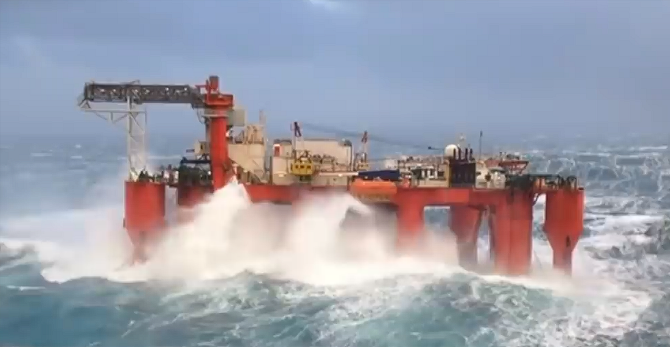
\includegraphics[height = 3cm]{figures/ch1-平台底部砰击.png}
		\caption{平台底部遭受波浪砰击}
    \label{fig:ch1-平台底部砰击}		
	\end{subfigure}
	\begin{subfigure}[b]{0.4\textwidth}
		\centering
		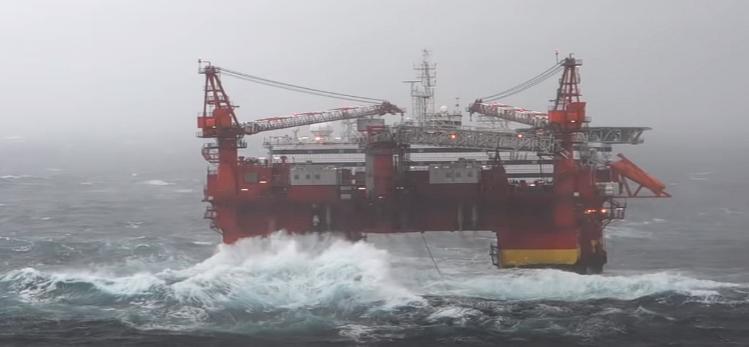
\includegraphics[height = 3cm]{figures/ch1-平台立柱砰击.png}
		\caption{平台立柱遭受波浪砰击}
    \label{fig:ch1-平台立柱砰击}
	\end{subfigure}
	\caption{北海石油钻井平台遭受波浪砰击(图片来自网络)}
	\label{fig:ch1-北油平台砰击}
\end{myfigure}

浮式平台所遭受的波浪砰击、上浪等强非线性作用会对平台造成严重危害。%
波浪砰击会产生极大的强非线性瞬时砰击载荷，对平台结构的安全性能是巨大的考验；%
而平台上浪可能会对甲板上的设施设备甚至人员安全造成威胁，引发严重的安全事故。%
因此对这类强非线性波浪结构物相互作用的问题进行研究和分析是十分必要的。%
然而这一类强非线性波浪结构物相互作用的问题一般涉及液面喷溅、空气卷吸以及结构运动等现象，%
属于气液固耦合的复杂动力学问题，一直以来都是船舶与海洋工程中的研究重点和难点\cite{faltinsenSlammingMarineApplications2004}。%
针对该问题，学者们提出了各种理论分析、数值模拟和试验研究方法。%
其中理论分析由于假设的高度简化，一般只适用于一些简单结构以及线性或弱非线性波浪结构物相互作用问题；%
而模型试验耗费大、周期长、对试验技术与设备的要求高，具有较大的局限性。%
相反地，数值模拟耗费小、周期短、受环境影响小且可获得更为丰富的流场信息，%
尤其是计算流体动力学(Computational Fluid Dynamics，简称CFD)方法能够有效处理复杂强非线性波浪结构物相互作用问题，%
现已逐渐成为研究这类问题的重要手段\cite{zhouNumericalModellingDynamic2019,%
paulsenProbabilityWaveSlamming2019,%
zhuExperimentalInvestigationBreaking2022,%
huoStudyWaveSlamming2023}。%

浮式平台与固定式平台不同，在畸形波、风暴潮等恶劣海况下会产生大幅度运动，%
该运动同时也会影响波浪运动和平台受力，从而形成一个复杂的动态耦合系统，%
使得结构物的运动响应和波浪载荷的准确预报更加困难\cite{张HaiYangJieGouWuBoLangPengJiDeShuZhiYanJiuZongShu2023}，%
如\cref{fig:ch1-动态耦合系统}所示。%
因此在对浮式平台波浪砰击、上浪等问题进行强非线性载荷数值预报时，%
需要同时考虑大尺度极端波浪的生成、波浪的辐射和绕射，%
平台近场小尺度区域的瞬态砰击、上浪过程，以及平台在波浪中的载荷和运动响应。%
\begin{myfigure}
	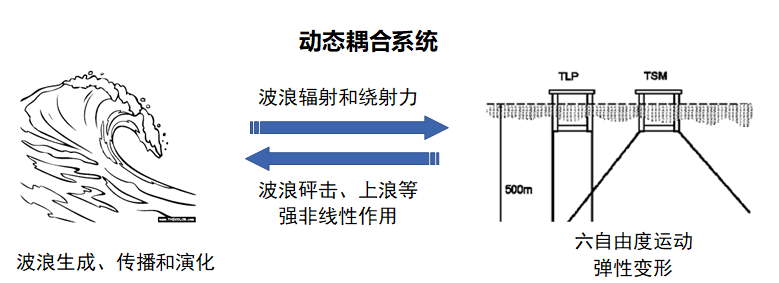
\includegraphics[width = 12cm]{figures/ch1-动态耦合系统.png}
	\caption{波浪-浮式平台动态耦合系统}
  \label{fig:ch1-动态耦合系统}
\end{myfigure}

\subsubsection{
  \texorpdfstring{数值方法需求} % 正文和目录中显示的标题
  {\thesubsubsection 数值方法需求} % 书签页中显示的标题
}
\label{sssec:数值方法需求}

对于波浪砰击、平台上浪这类局部存在大梯度流场和大变形自由液面的强非线性相互作用问题，%
采用VOF(Volume of Fluid)方法捕捉自由液面的有限体积法(Finite Volume Method，简称FVM)%
\cite{xieNumericalPredictionSlamming2018,bilandiNumericalSimulationVertical2018a}%
和无网格的光滑粒子流体动力学(Smoothed Particle Hydrodynamics，简称SPH)%
\cite{ogerTwodimensionalSPHSimulations2006a,%
shaoIncompressibleSPHSimulation2009,%
gaoNumericalModellingRegular2012a,%
sunSuctionEffectFreak2019}相对于其他数值方法更具有优势\cite{张HaiYangJieGouWuBoLangPengJiDeShuZhiYanJiuZongShu2023}。%

现有的强非线性波浪浮式平台相互作用数值研究主要集中于水槽/水池计算，%
多采用FVM方法进行流场离散，并通过VOF方法捕捉自由面。%
Liang等人\cite{liangNumericalStudyAir2010}%
通过VOF两相流求解器以及DNV船级社强度分析软件SESAM中的深水浮式系统锚泊耦合分析DeepC模块，%
对不规则波浪中处于系泊状态下的半潜式平台进行了波浪砰击的气隙响应研究。%
刘亚秋\cite{刘BanQianShiPingTaiDuoLiZhuBoLangPaShengYuPengJiTeXingYanJiu2019}%
使用CFD软件FINE/Marine对半潜式平台立柱的波浪爬升问题进行研究，%
主要分析了波浪参数对爬升现象的影响，并且研究了立柱参数对平台波浪爬升的影响。%
安康等人\cite{安TuoHangGongKuangXiaBanQianPingTaiChengGanDuiBoLangPengJiDeMinGanXing2020,%
施TuoHangGongKuangXiaBanQianShiPingTaiHengChengBoLangPengJiTeXingShiYanYanJiu2021}%
采用动网格法和VOF两相流求解器对拖航工况下半潜平台撑杆的砰击问题进行了研究，%
包括不同测点位置、不同流速和浪向角下的砰击特性等。%
Yao等人\cite{yaoExperimentalNumericalInvestigation2023a}通过StarCCM+中的VOF方法追踪自由面以及六自由度动态耦合%
(Dynamic Fluid Body Interaction，简称DFBI)模型定义系泊缆和平台的运动，对恶劣海况下的半潜式平台进行了数值模拟。%

近年来，基于无网格描述的CFD方法在模拟强非线性波浪结构物相互作用方面受到了广泛的关注。%
Rudman和Cleary等人\cite{rudmanRogueWaveImpact2009,rudmanRogueWaveImpact2013,rudmanInfluenceMooringSystem2016}%
采用基于无网格描述的SPH法对极端环境下半潜式平台的水动力特性进行了数值研究，%
先后探究了不同系泊系统的浮式平台在波浪砰击作用下的运动响应，%
以及波浪入射角与系泊缆预张力对张力腿平台(Tension Leg Platfomathrm，简称TLP)运动幅值和系泊缆最大张力及松弛度的影响。%
研究表明，与有网格CFD技术相比，SPH法可以更有效地处理波浪破碎、波浪与结构物的强非线性相互作用等问题。%
值得注意的是在他们的计算中，物理时间80秒，需要单核CPU运行300小时。%
Pan等人\cite{panApplicationSPHMethod2016a}采用SPH方法对溃坝下游立方柱的砰击力以及极端波浪作用下的浮式平台的运动进行了计算，%
波浪与浮体相互作用的数值模型及计算结果如\cref{fig:ch1-TPL-SPH模拟}所示。%
\begin{myfigure}
	\begin{subfigure}[b]{0.6\textwidth}
		\centering
		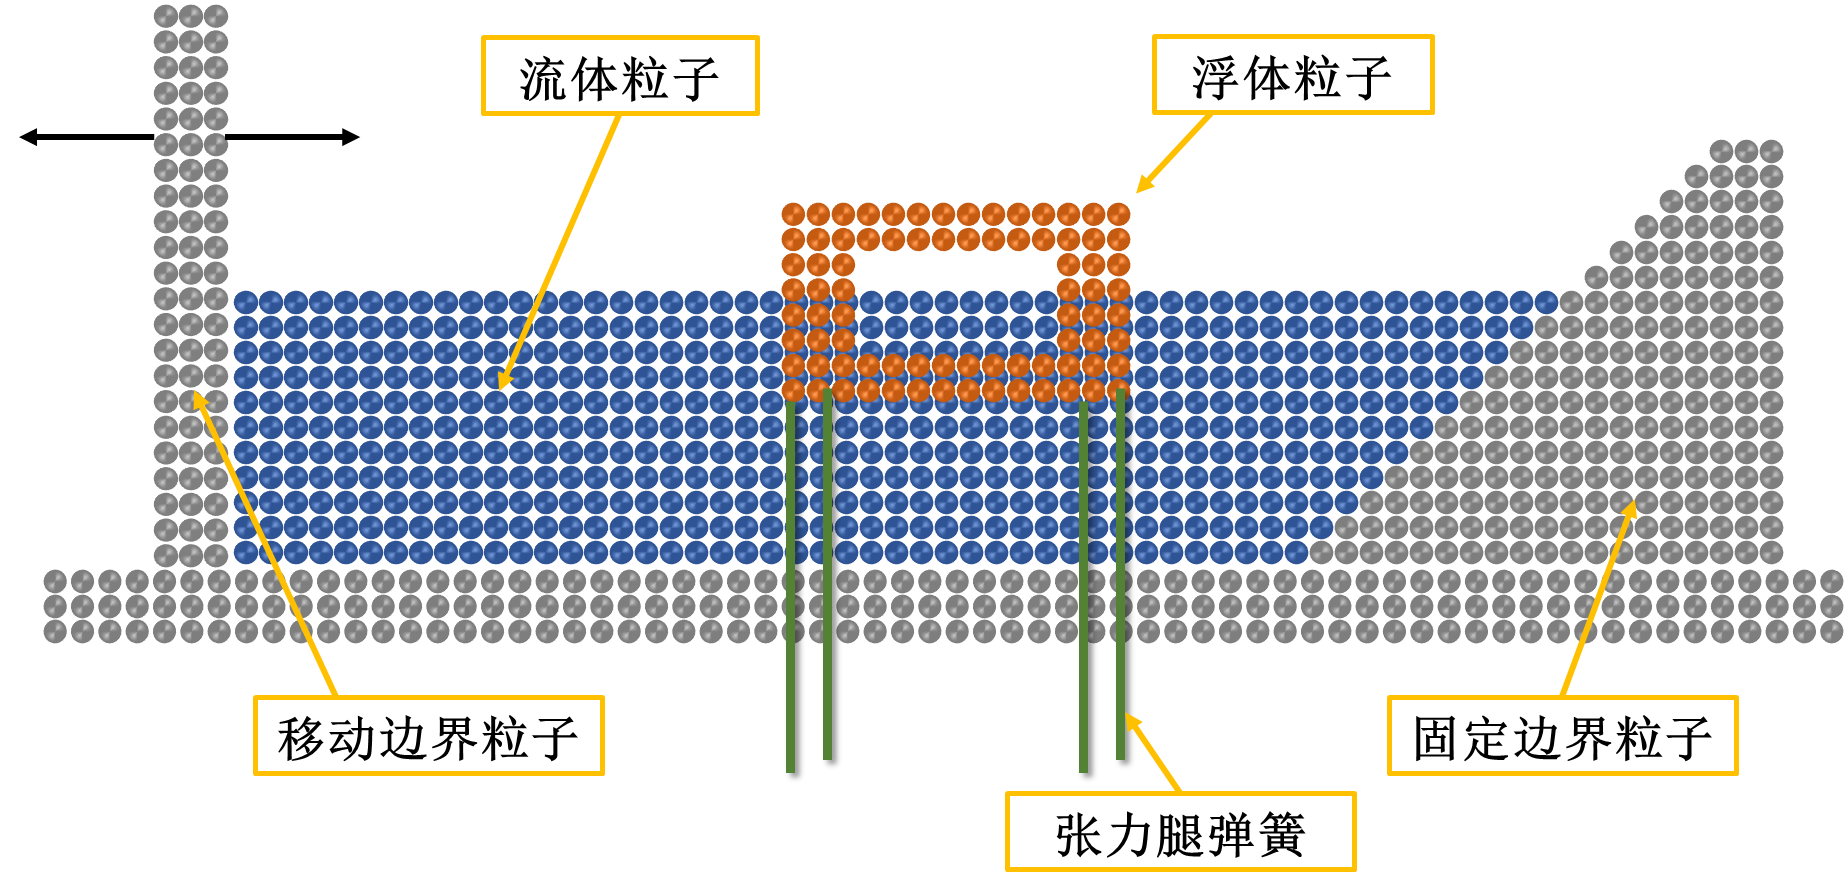
\includegraphics[width=\textwidth]{figures/ch1-TPL-SPH模型.png}
		\caption{极端波浪冲击平台的SPH数值模型}
    \label{fig:ch1-TPL-SPH模型}		
	\end{subfigure}
	\vspace*{3pt} % 调整竖直间隔
	\begin{subfigure}[b]{0.6\textwidth}
		\centering
		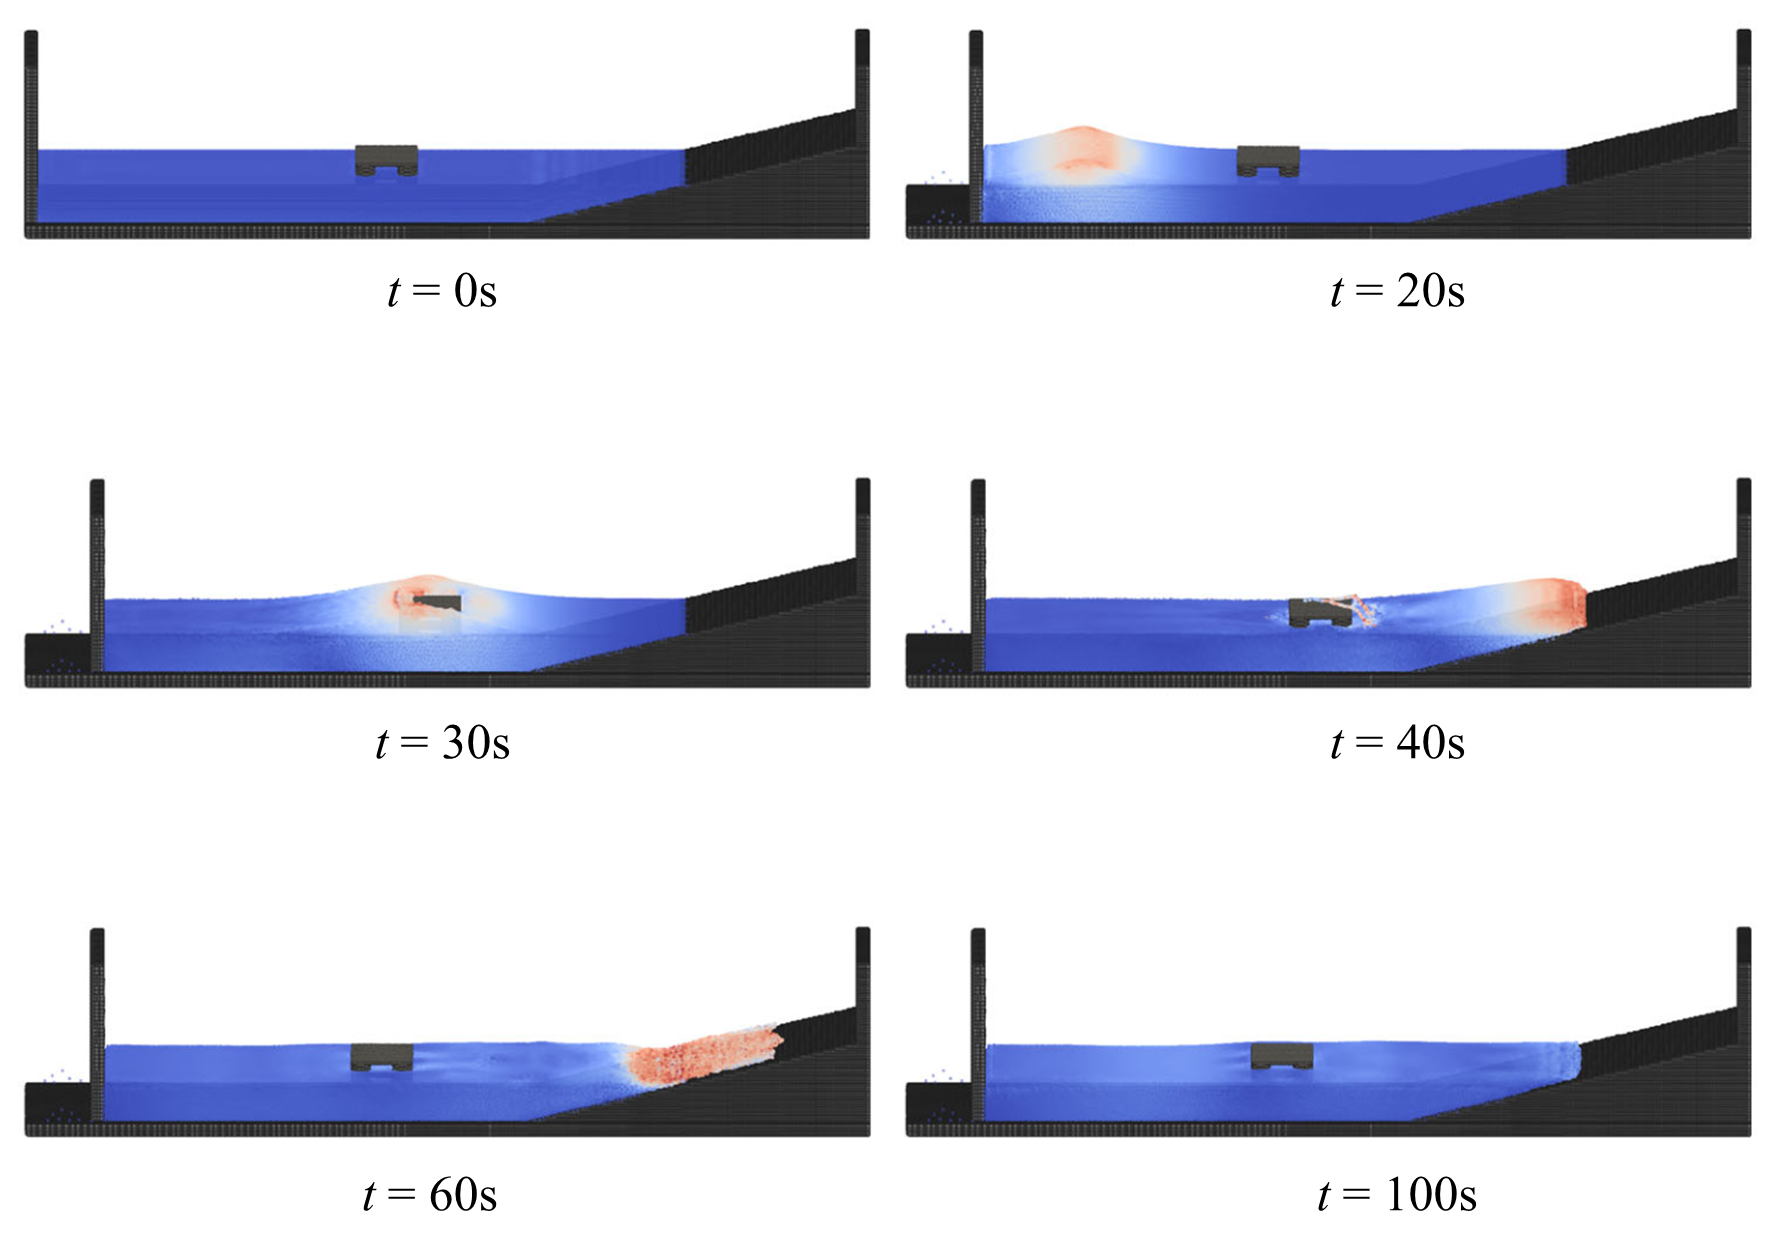
\includegraphics[width=\textwidth]{figures/ch1-TPL-结果.png}
		\caption{SPH模拟结果快照}
    \label{fig:ch1-TPL-结果}
	\end{subfigure}
	\caption{TLP波浪砰击的SPH方法数值计算模型及计算结果\cite{panApplicationSPHMethod2016a}}
	\label{fig:ch1-TPL-SPH模拟}
\end{myfigure}

数值结果和试验结果对比表明，SPH方法可以准确捕捉重力和惯性力驱动流中固定物体的复杂瞬态载荷特性以及浮式平台的刚体运动。%
此外他们对聚焦波下TLP的运动进行了数值模拟，并且将张力腿假设为弹簧模型，详细地分析了波浪冲击力以及张力腿所施加的反作用力。

研究人员对势流边界元方法和CFD方法在波浪浮式平台相互作用数值模拟方面进行了对比，%
发现势流方法的计算速度远远高于CFD方法，%
而CFD方法在受到粘性和强非线性因素影响较大的流场计算中更加准确。%
Rivera-Arreba等人\cite{rivera-arrebaModelingSemisubmersibleFloating2019}%
和Zhou等人\cite{zhouInvestigationFocusedWave2019}%
对比了势流方法和CFD方法在计算波浪中半潜式风机平台的运动响应和波浪力时的表现。%
其中，Rivera-Arreba等人\cite{rivera-arrebaModelingSemisubmersibleFloating2019}%
采用了基于势流理论的二阶边界元势流求解器和基于Navier-Stokes(NS)方程的VOF方法的两相流求解器，%
计算结果表明对于波陡不大的规则波，两种数值模拟方法均能很好地模拟结构物的响应；%
而对于大波陡波浪，由于势流求解器不能考虑粘性以及高阶非线性的影响，两种模型的计算结果存在差别。%
类似地，Zhou等人\cite{zhouInvestigationFocusedWave2019}在浮式风机平台的水动力计算中，%
通过对一阶、二阶势流结果以及CFD结果的对比分析，发现势流计算和CFD计算在靠近结构自然频率时的结果有很大的差别。%
在他们的工作中CFD部分的网格数量为235.4万，在360核CPU并行运算下，80小时能够完成200秒物理时间的模拟，%
而势流软件只需要40秒便可完成相应的物理计算。%

对于复杂构型浮式平台的波浪砰击、上浪等问题，采用VOF方法的FVM方法和SPH方法是现在普遍采用的数值手段。%
SPH方法相较于FVM方法得益于其拉格朗日和无网格粒子特性，对于自由液面或流固界面可自动完成追踪，并且精确满足质量守恒，%
因此比较适合于模拟强非线性作用过程中的液体喷溅和结构大幅运动等自由液面大变形和动边界过程。%
但是由于CFD方法的计算成本限制，对强非线性波浪浮式平台相互作用问题的数值模拟远远达不到工程需要。%

总的来说，在对波浪与浮式平台的强非线性作用进行数值预报时，%
需要同时考虑大尺度极端波浪的生成和演化、波浪的辐射和绕射，%
平台近场小尺度区域强非线性过程以及平台在波浪中的运动响应。%
基于势流理论的传统水动力分析方法难以准确计算强非线性流固耦合问题，%
而CFD方法由于计算量大且格式耗散性强等原因无法长时间准确捕捉波浪运动。%
因此，根据势流方法和CFD方法的特点，结合两者优势的势粘流耦合方法逐渐被关注。%
自上世纪八十年代以来，不少学者对势粘流耦合方法进行了探索和研究，%
然而对于耦合区域或耦合界面的处理尚存在诸多难点，%
同时对于实际工程中出现的开放海域砰击问题的研究依然处于起步阶段\cite{choiGrid2GridHOSWrapper2017}，%
因此建立一种能够模拟强非线性波浪浮体相互作用问题的高效求解器是十分必要的。%

综上，本文旨在面向海洋工程中的浮式平台遭受波浪强非线性作用这一问题背景，%
对势粘流耦合方法展开初步研究，以探索能够实现精细高效模拟波浪与浮式平台强非线性相互作用的可行方法，%
从而为后续工程应用中海上浮式平台的安全性评估和结构优化设计提供数值方法支撑。%

\subsection{
  \texorpdfstring{势粘流耦合方法研究现状} % 正文和目录中显示的标题
  {\thesubsection 势粘流耦合方法研究现状} % 书签页中显示的标题
}
\label{ssec:势粘流耦合方法研究现状}

数值模拟作为波浪与结构物相互作用研究的一种重要手段，被广泛应用于船舶与海洋工程水动力研究中。%
本文重点关注非线性波浪的生成和演化以及波浪与结构物相互作用两类问题的数值模拟方法。%
在数值模拟中，首先需要考虑非线性波浪的生成、长时间大尺度的传播演化，%
以及在波浪演化或与结构物作用过程中小尺度范围内可能发生的波浪破碎、空气卷吸等现象。%
此外，对于波浪与结构物相互作用问题，还需要考虑结构物壁面附近的流体粘性效应和有旋流动。%
要准确地对波浪与结构物相互作用问题进行模拟，需要考虑多尺度流动、非线性波浪、水气两相流以及粘性旋度等因素。%

在粘性、旋度等因素可忽略时，波浪的生成和演化以及波浪与结构物的相互作用问题可以通过势流理论进行求解。%
边界元方法\cite{hessCalculationNonliftingPotential1964,贺JianDanGreenHanShuFaQiuJieSanWeiShuiDongLiXiShu1986}、%
水弹性理论\cite{priceHydroelasticityMarineStructures1985,田ChuanBoShuiDanXingLiXueLiLunDeYanJiuJinZhan2008}%
等都基于势流理论对波浪中船舶和海上平台的动力响应进行分析，%
并且许多势流模型已经发展出了非线性理论，能够处理弱非线性\cite{袁ShenHaiFuShiJieGouWuXiBoXiTongDeFeiXianXingShiYuFenXi2011}%
甚至完全非线性\cite{sunTwoDimensionalFully2012a}问题。%
理论上，在无粘无旋且不可压缩流体假设下，势流理论的控制方程由NS方程简化为Laplace方程。%
通过半解析的势流方法进行求解时，问题在空间维度上被降阶因此能极大减小计算量，且对于开放域问题具有优势。%
同时由于势流模型的数值耗散低，在对大尺度波浪的生成和演化这一类问题进行模拟时计算精度和效率都较高。%
但是由于对流动进行了高度简化，势流理论无法解决复杂问题，如船舶的粘性阻力、涡激力、结构物周围的流动分离以及波浪破碎等。%

CFD方法，主要通过求解NS方程来模拟波浪与结构物相互作用的问题。%
CFD方法能够在模拟过程中考虑粘性、旋度以及湍流等，%
并且通过一些自由面捕捉方法如水平集方法\cite{sussmanLevelSetApproach1994} (Level Set Method，简称LSM)、%
VOF\cite{hirtVolumeFluidVOF1981} (Volume of Fluid，简称VOF)等可实现对两相流的模拟，%
因此采用CFD方法模拟波浪与结构物相互作用问题，%
能够更加精确地反映流动细节和结构物响应\cite{tezdoganFullscaleUnsteadyRANS2015,oggianoReproductionSteepLong2017,songValidationCFDApproach2020}。%
相应地，CFD方法相较于势流模型对计算资源的需求更大，当问题涉及的时空尺度较大且对精度要求较高时更是如此。%
同时，CFD方法的数值耗散较大，不适合进行长时间、大尺度波浪问题的模拟。%

Ransley等人\cite{ransleyBlindComparativeStudy2019,ransleyBlindComparativeStudy2020}%
的盲测中比较了几种CFD求解器和势流求解器对无破碎波浪与结构物相互作用问题的计算结果。%
在中等波陡波浪条件下，即使是最快的CFD求解器也比势流求解器慢1.5个数量级。%
但作者同时提出，如果势流理论的假设不再成立，即当波陡增大至波浪发生破碎时，只有使用CFD求解器才能很好地解决问题。%

船舶与海洋工程水动力研究中所涉及的流动问题一般为高雷诺数流动，流体的粘性主要作用于结构物面附近的薄层—即边界层内部，%
而边界层外部的流动由于能量耗散，其旋度和粘性影响在远离近场时会逐渐减小直至消失，可近似为无旋理想流动。%
因此在靠近结构物的内域采用CFD方法求解，而在远离结构物的外域采用势流方法求解，%
从而通过不同的模型来更高效地模拟不同的物理现象是十分自然的想法。%
在过去的几十年间有诸多学者对势粘流耦合进行了探索和研究，发展了许多不同的模型和方法，并且已将这些方法应用到各类问题中。%
下文将简述这两类势粘流耦合方法。%

\subsubsection{
  \texorpdfstring{区域分解方法} % 正文和目录中显示的标题
  {\thesubsubsection 区域分解方法} % 书签页中显示的标题
}
\label{sssec:区域分解方法}

区域分解方法是最早被用于进行势粘流耦合研究的方法。%
自二十世纪初Prandtl\cite{prandtlUberFlussigkeitsbewegungBei1904}提出边界层理论以来，学者们对粘流和无粘流间的耦合展开了诸多研究。%
在边界层理论中，流体的粘性效应主要体现在边界层内部，而在边界层外部流动可近似视为无粘流或理想流动。%
与边界层理论类似，区域分解方法的基本思路是将流域划分为势流域$\Omega_{\rm{PF}}$和粘流域$\Omega_{\rm{NS}}$，在不同流域采用不同的模型进行求解，并%
在耦合区域$\Omega_{\rm{Coupling Domain}}$或耦合界面$\Gamma_{\rm{Coupling}}$处进行耦合计算，%
以实现势流与粘流的耦合过程，如\cref{fig:ch1-DD-示意图}所示。
\begin{myfigure}
	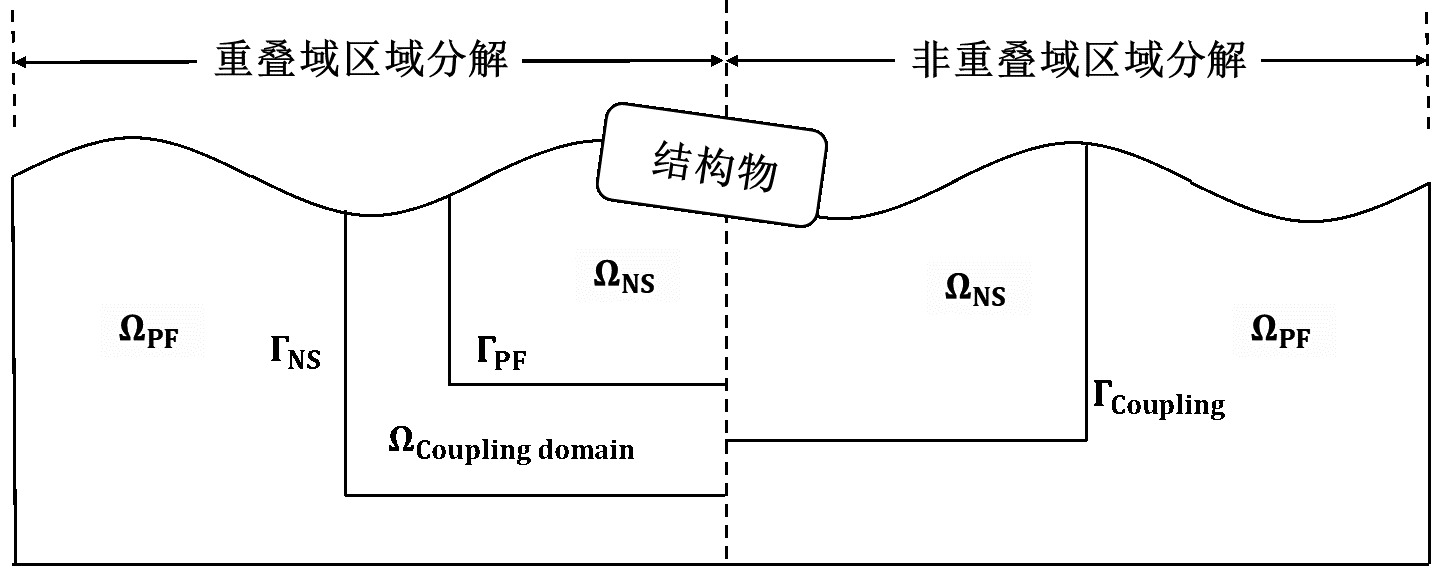
\includegraphics[width = 12cm]{figures/ch1-DD-示意图.png}
	\caption{区域分解方法示意图}
	\label{fig:ch1-DD-示意图}
\end{myfigure}

区域分解方法的关键在于势粘流模型、耦合方法和流域划分这三个方面，下文将对此展开介绍。%

(1)	势粘流模型%

势流理论是基于不可压、无粘、无旋假设建立的，其流动可以通过速度势描述，控制方程为Laplace方程；%
粘流方法的基本控制方程为连续性方程和NS方程，能够考虑流体的可压缩性和粘性效应。%

\cref{tab:ch1-DD-PFNS-models}中列举了一些以往区域分解方法研究中所采用的势粘流模型。%

\begin{mytable}
	\caption{区域分解方法中的势粘流模型}
	\label{tab:ch1-DD-PFNS-models}
	\begin{tabularx}{\textwidth}{c|c|X}
		\toprule
		{势粘流模型} & \multicolumn{2}{c}{方法类型} \\
		\midrule
		\multirow{11}{*}{势流模型} & \multirow{2}{*}{势流波浪模型} & {Boussinesq模型\cite{narayanaswamyHybridBoussinesqSPHWave2008,%
		christensenTransferBoussinesqWaves2009,kassiotisCouplingSPH1D2011,weiCostEffectiveMethodModelling2017}} \\
		& & {SWASH模型\cite{altomareCouplingSWASHSPH2014} (Simulating WAves till SHore model)} \\
		\cline{2-3}
		& \multirow{9}{*}{势流数值方法} & {边界元法\cite{campanaDomainDecompositionFree1994,campanaViscousinviscidCouplingFree1995,%
		guignardComputationShoalingBreaking1999,iafratiDomainDecompositionApproach2003,lachaumeModelingBreakingPostbreakingWaves2003,%
		biausserNumericalAnalysisInternal2004,drevardExperimentalValidationCoupled2005,colicchioBEMlevelSetDomaindecomposition2006,%
		kimSimpleTwowayCoupling2010,zhangCouplingViscousPotential2013,zhangSolitaryWaveBreaking2015,%
		孟JiYuShuangXiangShiLiuNianLiuOuHeDeShuZhiXiaoBoMoNi2022,sunWeakCouplingMPS2017,%
		taoApplicationAdvancedCoupled2022b} (Boundary Element Method，简称BEM)} \\
		& & {高阶谱法\cite{ogerCoupledSPHspectralMethod2014,nelliExperimentalNumericalModels2017,zhuangRegularIrregularWave2018,%
		choiGenerationRegularIrregular2018,韩ZhiLiYuanZhuBoLangPaShengHOSCFDShuZhiMoNi2019,%
		宋JiYuGaoJiePuFangFaYuCFDJiSuanDeOuHeMoXingZaiBuGuiZeBoMoNiZhongDeYingYong2019,%
		宋JiYuGaoJiePuFangFaYuCFDOuHeMoXingDeJiDuanBoLangShuZhiMoNi2019,庄GaoJiePuFangFaYuCFDFangFaOuHeDeShuZhiMoNiJiShu2019,%
		郭JiYuNianXingLiuHeNianShiLiuOuHeFangFaDeChuanBoBoLangZengZuYuYunDongXiangYingShuZhiYanJiu2020,%
		韩JiYuHOSCFDNianShiLiuOuHeFangFaMoNiZhiLiYuanZhuBoLangPaSheng2021,zhuangParametricStudyNew2021} (High Order Spectral，简称HOS)} \\
		& & {有限体积法\cite{kristiansenGapResonanceAnalyzed2012,luOverlappingDomainDecomposition2017} (Finite Volume Method，简称FVM)} \\
		& & {有限元法\cite{glowinskiDomainDecompositionMethods1983,dinhCouplingViscousInviscid1988,kimRingingAnalysisVertical2012,%
		baquetNumericalModelingUsing2017} (Finite Element Method，简称FEM)} \\
		& & {有限差分法\cite{paulsenEfficientDomainDecomposition2014,钟JiYuShiLiuNianLiuShuangXiangOuHeMoXingDeShuZhiZaoBo2022,%
		agarwalThreedimensionalCouplingBoussinesq2022} (Finite Difference Method，简称FDM)} \\
		& & {准拉格朗日欧拉有限元法\cite{liZonalHybridApproach2018,yanNumericalSimulationWave2019,zhang3DHybridModel2019,%
		zhang3DHybridModel2020,zhangNumericalStudyInteraction2021} (Quasi Lagrangian Eulerian Finite Element Method，简称QALE-FEM)} \\
		& & {无旋层析水波理论\cite{赵JiYuShiNianLiuDanXiangOuHeDeKCSBoLangZengZuYanJiu2018,%
		ZhaoShiNianLiuDanXiangOuHeDeZhiLiYuanZhuBoLangPaShengMoNi2019} (Irrotational Green-Naghdi，简称IGN)} \\
		& & {调和多项式单元法\cite{robauxAssessmentOnewayCoupling2022} (Hamathrmonic Polynomial Cell，简称HPC)} \\
		\hline
		\multirow{7}{*}{粘流模型} & \multirow{2}{*}{有网格方法} & {FVM\cite{narayanaswamyHybridBoussinesqSPHWave2008,%
		campanaViscousinviscidCouplingFree1995,guignardComputationShoalingBreaking1999,iafratiDomainDecompositionApproach2003,%
		lachaumeModelingBreakingPostbreakingWaves2003,biausserNumericalAnalysisInternal2004,drevardExperimentalValidationCoupled2005,%
		kimSimpleTwowayCoupling2010,孟JiYuShuangXiangShiLiuNianLiuOuHeDeShuZhiXiaoBoMoNi2022,nelliExperimentalNumericalModels2017,%
		zhuangRegularIrregularWave2018,choiGenerationRegularIrregular2018,韩ZhiLiYuanZhuBoLangPaShengHOSCFDShuZhiMoNi2019,%
		宋JiYuGaoJiePuFangFaYuCFDJiSuanDeOuHeMoXingZaiBuGuiZeBoMoNiZhongDeYingYong2019,庄GaoJiePuFangFaYuCFDFangFaOuHeDeShuZhiMoNiJiShu2019,%
		郭JiYuNianXingLiuHeNianShiLiuOuHeFangFaDeChuanBoBoLangZengZuYuYunDongXiangYingShuZhiYanJiu2020,%
		韩JiYuHOSCFDNianShiLiuOuHeFangFaMoNiZhiLiYuanZhuBoLangPaSheng2021,zhuangParametricStudyNew2021,kristiansenGapResonanceAnalyzed2012,%
		luOverlappingDomainDecomposition2017,glowinskiDomainDecompositionMethods1983,kimRingingAnalysisVertical2012,%
		paulsenEfficientDomainDecomposition2014,钟JiYuShiLiuNianLiuShuangXiangOuHeMoXingDeShuZhiZaoBo2022,liZonalHybridApproach2018,%
		赵JiYuShiNianLiuDanXiangOuHeDeKCSBoLangZengZuYanJiu2018,ZhaoShiNianLiuDanXiangOuHeDeZhiLiYuanZhuBoLangPaShengMoNi2019,%
		robauxAssessmentOnewayCoupling2022,hildebrandtSimulationFocusingWaves2013,liNumericalSimulationFocusing2018,%
		junxianModellingFocusedWave2020}} \\
		& & {FEM\cite{zhangCouplingViscousPotential2013,zhangSolitaryWaveBreaking2015,glowinskiDomainDecompositionMethods1983,%
		dinhCouplingViscousInviscid1988,hamiltonViscousinviscidMatchingWave2002}} \\
		\cline{2-3}
		& \multirow{5}{*}{无网格方法} & {光滑粒子流体动力学方法\cite{kassiotisCouplingSPH1D2011,altomareCouplingSWASHSPH2014,%
		weiCostEffectiveMethodModelling2017,taoApplicationAdvancedCoupled2022b,ogerCoupledSPHspectralMethod2014,%
		zhang3DHybridModel2019,zhang3DHybridModel2020,zhangNumericalStudyInteraction2021} (Smoothed Particle Hydrodynamics，简称SPH)} \\
		& & {移动粒子半隐式方法\cite{sunWeakCouplingMPS2017} (Moving Particle Semi-implicit，简称MPS)} \\
		& & {Rankine源无网格Petrov-Galerkin法\cite{agarwalThreedimensionalCouplingBoussinesq2022,sriramHybridMethodModelling2014,%
		kumarHybridNumericalModel2020} (Meshless Local Petrov-Galerkin method with Rankine Source，简称MPLG\_R)} \\
		\bottomrule
	\end{tabularx}
\end{mytable}

常用的势流模型主要为BEM和HOS方法。%
BEM作为一种半解析方法，能够将体网格计算转化为面网格计算，因此求解精度和计算效率都较高，并且适合处理开放边界问题。%
HOS方法作为一种伪谱法，在数值计算中引入了快速傅里叶变换，因此计算效率高且数值耗散低，适合长时间大尺度的波浪演算。%
粘流模型常用FVM方法离散流域，该方法守恒性好，网格对复杂几何区域的适应性强，并可通过VOF模型追踪自由面实现两相流的求解。%
SPH作为一种无网格方法，得益于其拉格朗日和无网格粒子特性，%
采用合适的离散格式即可实现自动捕捉自由液面\cite{colagrossiTheoreticalConsiderationsFreesurface2009}，%
并且精确满足质量守恒，因而在砰击、上浪等强非线性自由面问题的势粘流耦合中也被广泛应用。%

(2) 耦合方法%

耦合方法是区域分解方法的研究重点。%
从势粘流域是否重叠考虑，有重叠域耦合和非重叠域(即界面)耦合；%
从耦合方向考虑，可以分为单向耦合和双向耦合，即势粘流域间的信息是单向传递还是双向传递，也称为弱耦合和强耦合；%
从匹配方式考虑，主要有迭代匹配和松弛函数两种方法；%
从匹配的边界条件考虑，更是丰富多样，例如速度势Dirichlet条件，速度法向分量Neumann条件等。%
值得注意的是，对于船舶与海洋工程中的水动力问题，由于自由面的存在，不同区域匹配时所用的边界条件是耦合准确性和稳定性的关键。%

最早区域分解方法被用于空气动力学的势粘流耦合研究。%
Dinh等人\cite{glowinskiDomainDecompositionMethods1983,dinhCouplingViscousInviscid1988}针对不可压粘性流问题，%
按照距离物面远近将流域分为外部势流域和内部粘流域，并在两者间保留有重叠区域。%
粘流域提供速度势作为势流域的Dirichlet边界条件，势流域为粘流域提供速度边界条件，子域间迭代运算至收敛，%
收敛条件为重叠域内的势流速度势梯度和粘流速度满足最小二乘优化条件。%
在二维机翼绕流问题的计算中，通过FEM对势粘流控制方程进行离散，耦合方法的粘流域节点和单元数量相较于全粘流方法减少近1/3，%
并且计算给出的机翼表面压力分布、流线图和涡量场也与后者吻合良好。%
不过由于收敛所需的迭代计算量并不小，因此对计算效率的提高并不明显。%

Campana等人\cite{campanaDomainDecompositionFree1994,campanaViscousinviscidCouplingFree1995}%
将势粘流耦合方法引入至船舶水动力性能预报的研究中。%
与Dinh等人\cite{dinhCouplingViscousInviscid1988}的方法不同，%
Campana等人\cite{campanaDomainDecompositionFree1994}尝试取消势粘流重叠区域，仅通过界面进行耦合。%
在界面处，粘流域提供速度法向分量作为势流域的Neumann边界条件，而势流域提供速度和压力作为粘流域边界条件。%
对定常流中几类船型的计算结果显示，尽管能够收敛，但收敛速度不是很理想，并且在界面上观察到了非平滑过渡。%
因此Campana等人\cite{campanaViscousinviscidCouplingFree1995}将界面改为重叠区域，%
势流域在粘流边界Гp仅提供速度作为边界条件，而粘流域在势流边界Гv提供边界条件不变，如下：%
\begin{equation}
	\left.\bm{u}\right|_{\Gamma_{\rm{v}}} = \nabla\left.\phi\right|_{\Gamma_{\rm{v}}}, \qquad
	\left.\left(\frac{\partial \phi}{\partial n}\right)\right|_{\Gamma_{\rm{p}}} = \bm{u}\cdot\left.\bm{n}\right|_{\Gamma_{\rm{p}}}
\end{equation}
式中：$\phi$为速度势，$\bm{u}$为速度，$\bm{n}$为边界法向。%
采用该方法对几类船型进行模拟计算，给出的压力云图与全粘流方法和试验数据对照都吻合较好，而计算时间仅为全粘流方法的1/6。%
新方法提高了收敛速度，并保证了匹配面上的平滑过渡，但艏艉处的计算结果较差，试验中观察到的速度场S形轮廓并未出现。%

进一步地，Iafrati和Campana\cite{iafratiDomainDecompositionApproach2003}针对界面耦合提出了新的耦合边界条件，%
并与Campana\cite{campanaViscousinviscidCouplingFree1995}的重叠域耦合方法进行了对比。%
势流域提供速度和压力边界条件，粘流域通过非稳态Bernoulli方程获得界面上的速度势，为势流域提供Dirichlet边界条件，在界面Г上的边界条件如下：%
\begin{equation}
	\bm{u}_{\rm{v}} = \nabla \phi,\quad 
	p_{\rm{v}} = p_{\rm{p}} - 2\mu \frac{\partial \bm{u}_n}{\partial n}, \quad
	\phi = \int_{0}^{t}\frac{\partial \phi}{\partial t} {\rm{d}} t 
	= \int_{0}^{t} \left(-\frac{p_{\rm{v}}}{\rho} - \bm{g} - \frac{\left|\bm{u}_{\rm{p}}\right|^2}{2}\right) {\rm{d}} t 
\end{equation}
式中：$\phi$为速度势，$\bm{u}_{\rm{p}}$、$\bm{u}_{\rm{v}}$、$p_{\rm{p}}$和$p_{\rm{v}}$分别为势粘流域的速度及压力，%
$\bm{n}$为边界法向，$\rho$为流体密度。新的界面耦合方法相较于重叠域耦合，收敛速度更快，但误差略大。%
采用该方法对浸没水翼产生的破碎波进行模拟，能够将粘流域大小缩小至计算域的30\%。%
Zhang等人\cite{zhangCouplingViscousPotential2013,zhangSolitaryWaveBreaking2015}%
在Iafrati等人\cite{iafratiDomainDecompositionApproach2003}的基础上提出了新的隐式迭代方法，%
并加入了自由面校正和不匹配网格插值，模拟的溃坝过程与试验吻合较为一致。

Hamilton等人\cite{hamiltonViscousinviscidMatchingWave2002}将外域无粘自由表面流在圆柱界面上的广义解用“壳函数”(Shell Functions)表达，%
使界面上的速度和压力通过“壳系数”(Shell Coefficients)相关联。%
并且提出了一种新的“压力驱动”耦合方法，内域依赖外域在界面上提供压力以进行下一步计算。%
预求解并存储“壳系数”后，内域只需要提供界面处的速度，就能够通过“壳函数”获得外域在界面上的压力，达到一次求解、多次使用，从而实现更高效的界面耦合。%
对规则波圆柱绕流的模拟结果显示，耦合方法较势流方法计算的波浪力较小。%
除了依靠显式传递边界条件实现势粘流耦合，Kristiansen等人\cite{kristiansenGapResonanceAnalyzed2012}在势粘流域均采用FVM数值方法，%
并将粘流求解过程分解，从而能够在整场流域得到一个单一的方程组，隐式包含了势粘流域边界条件的交互。

孟巍等人\cite{孟JiYuShuangXiangShiLiuNianLiuOuHeDeShuZhiXiaoBoMoNi2022}结合松弛函数\cite{paulsenEfficientDomainDecomposition2014}%
和边界条件传递\cite{campanaDomainDecompositionFree1994}以实现双向耦合，%
即势流域向粘流域通过松弛函数传递波高和速度，而粘流域为势流域提供Neumann边界条件。%
通过该耦合方法实现的数值消波能够将粘流消波区减小为全粘流的1/5。%
钟文杰等人\cite{钟JiYuShiLiuNianLiuShuangXiangOuHeMoXingDeShuZhiZaoBo2022}采用了类似的方法，%
但松弛函数被用于粘流域向势流域传递波高和速度，而势流域在粘流域边界插值提供波高和速度条件。%
通过该方法实现的数值造波，能够在波浪传播接近粘流域入口时才开始粘流计算，进而节省计算时间。

上述耦合方法主要被用于波浪模型或势流数值方法等与有网格CFD方法间的耦合，%
而关于无网格CFD如光滑粒子流体动力学(Smoothed Particle Hydrodynamics，SPH)的耦合方法也有一定的发展。%
Narayanaswamy\cite{narayanaswamyHybridBoussinesqSPHWave2008}采用%
类似重叠区域耦合\cite{campanaViscousinviscidCouplingFree1995}的方式%
实现了Boussinesq波浪模型和SPH方法的耦合，对孤立波传播的模拟效果较好。%
Altomare等人\cite{altomareCouplingSWASHSPH2014}设置了一组速度由SWASH模型提供的SPH粒子，%
其形状在每一时间步变化，起到“造波桨”(Wave Paddle)的作用。%
通过这组“造波桨”粒子与自由流体粒子相作用而产生波浪，将势流域信息传递至粘流域中，实现了SWASH模型与SPH方法的单向耦合。%
该方法对规则波近岸浅化的模拟与试验结果对比一致性较好。%
Oger等人\cite{ogerCoupledSPHspectralMethod2014}在每一时间步，使用HOS方法将速度和压力赋给势粘流重叠域内的粒子，%
随后这些“受迫粒子”与粘流域内的“自由粒子”共同参与SPH计算以实现耦合。%
这里与Altomare等人\cite{altomareCouplingSWASHSPH2014}的方法不同，重叠域内的粒子会流入流出该区域，而非是固定的一组粒子，%
因此可以直接模拟波浪中水体的流动，而非通过造波桨\cite{altomareCouplingSWASHSPH2014}的移动产生波浪。

根据上述研究可知，耦合方法可以大致分为三类，\cref{tab:ch1-DD-models-characters}中简单总结了这几类常用耦合方法的部分特点。%
而边界条件的选取、耦合方向等方法细节在不同的研究中都有所不同，%
并且对于无网格粒子法有特殊的耦合方法，这些都要视具体问题而定。%
总而言之，耦合方法的关键在于精确地在势粘流域间传递流场信息(如速度、压力和波高等)，%
并且尽可能保证过渡区的平滑，解决在边界处可能出现的反射和发散等问题。
\begin{mytable}
	\caption{几类常用区域耦合方法的特点}
	\label{tab:ch1-DD-models-characters}
	\begin{tabularx}{\textwidth}{M{3.1cm} X X}
		\toprule
		{耦合方法} & {\centering 简介} & {\centering 特点} \\
		\midrule
		{重叠域迭代匹配} & {势粘流域互相在重叠域边界上提供边界条件，迭代计算至收敛} %
		& {势粘流域间过渡平滑，耦合精度较高；收敛速度较慢，计算效率提高不大} \\
		{界面迭代匹配} & {势粘流域在交界面处提供边界条件，迭代计算至收敛} %
		& {收敛速度较快，计算效率提高较大；势粘流域间过渡有间断，耦合精度略低}\\
		{重叠域松弛函数} & {通过重叠区域和松弛函数实现流场信息的传递} %
		& {无需迭代计算，对计算效率提高较大，松弛函数避免了反射波；非物理的耦合方法} \\
		\bottomrule
	\end{tabularx}
\end{mytable}

(3) 流域划分

在区域分解方法中，流域划分主要涉及势粘流域边界划分、势粘流域是否重叠、耦合区域的大小和位置或耦合界面的位置这几个问题，%
其中重叠区域在耦合方法中已经介绍，不在此赘述。其中，势粘流域边界划分将影响进出口边界、自由液面、物面等边界条件的处理。%

文献中对于流固耦合问题一般采用类似Campana等人\cite{campanaDomainDecompositionFree1994}的处理，%
将流域划分为结构物近场的粘流域和远场的势流域，自由面在势粘流域中都有分布。%
与之不同的是将自由面只包含于势流域或粘流域，例如Iafrati等人\cite{iafratiDomainDecompositionApproach2003}为了捕捉产生的波浪破碎现象，%
将流域上下划分，自由液面被完全包含于粘流域中，而浸没水翼在势流域中；%
Kristiansen等人\cite{kristiansenGapResonanceAnalyzed2012}将自由液面完全置于势流域内，%
仅将结构物底部发生流动分离的区域部分划为粘流域，因此他们的方法难以解决强非线性自由面问题。%

对于波浪生成和演化的流域划分，现有的研究主要关注强非线性自由面现象和数值波浪模拟两类。%
对于强非线性自由面问题，粘流域一般将强非线性现象发生的区域包含在内，%
如Guignard等\cite{guignardComputationShoalingBreaking1999}和%
Zhang等\cite{zhangCouplingViscousPotential2013,zhangSolitaryWaveBreaking2015}。%
对于数值波浪模拟问题，一般将势流域分布在粘流域的进出口以实现耦合造波或消波，%
如Baquet等\cite{baquetNumericalModelingUsing2017}和孟巍等\cite{孟JiYuShuangXiangShiLiuNianLiuOuHeDeShuZhiXiaoBoMoNi2022}。%

耦合区域的大小和位置或耦合界面的位置对于区域分解方法是一个较为复杂的问题，既要尽可能减小粘流域尺寸以提高计算效率，%
又需要保证粘流域的大小足以准确反映流动的粘性效应和强非线性现象等，并且需要考虑辐射波、绕射波的充分演化。%
Campana等人\cite{campanaViscousinviscidCouplingFree1995}对定常流中的S60船型进行模拟，%
耦合区域到船体的距离分别被设置为船长的1/20和1/100，其波高计算结果差距不大，这可能是由于该问题的非线性和粘性效应较弱。%
Iafrati等人\cite{iafratiDomainDecompositionApproach2003}对重叠域耦合的耦合区域宽度和界面耦合的界面位置都作了一定研究。%
当耦合区域的宽度较大时，不仅精度提高，收敛速度也有所增加。耦合界面的位置对速度结果影响较小，对波高几乎没有影响。%

Kim等人\cite{kimSimpleTwowayCoupling2010}针对BEM-FVM双向耦合方法，分析了耦合区域的宽度以及到结构物的距离对计算的影响。%
耦合区域宽度对波浪的计算结果影响并不大，并且除了波陡最小的一组试验，耦合方法的误差普遍小于全粘流方法。%
研究结论显示耦合区域到结构物的距离对一阶波幅影响不大，当距离为0.2和0.4倍波长时二阶波幅有较大差异，但当距离大于0.8倍波长时影响基本上消失。%
因此Kim等人\cite{kimSimpleTwowayCoupling2010}给出耦合区域到结构物的合适距离约为1.0倍波长。%
然而作者同时指出，流场中涡旋的强度可能由于波浪与结构物之间相互作用的强度而有所不同。因此对于不同问题，在选取该距离时还需要进一步的考虑。%

Zhuang等人\cite{zhuangParametricStudyNew2021}对基于松弛函数耦合的HOS-CFD单向耦合进行了较为丰富的参数化分析，%
其中也讨论了粘流域大小对计算的影响。通过对比三种大小的粘流域计算结果可以知道，当粘流域较小时船体周围的散射波无法充分演化，并且会出现更严重的反射波。%

区域分解方法通过将流域划分为不同子域，在子域内采用合适的模型进行求解，并通过重叠区域或界面实现子域间的信息匹配。%
因此对于区域分解方法来说，关键在于针对不同的问题和感兴趣的部分选择合适的耦合方法和势粘流模型。%
例如，对于波浪与结构物相互作用的问题，如果主要关心结构物的动力响应而忽略流场的细节，一般选择单向耦合。%
近几年研究者们倾向于采用松弛函数的耦合方法，而非通过迭代运算进行匹配耦合。%
这样做的好处是能够大幅减小计算量，避免了子域内重复的迭代运算，但是需要采取一定的手段以避免计算结果发散。%
此外，研究人员们对势粘流模型的选择十分多样，不同类型的问题需要选择合适的势粘流模型进行组合求解。

总的来说，基于区域分解的势粘流耦合方法经过一段时间的探索，已经在许多工程问题中得到了检验，\cref{tab:ch1-DD-progress}中列举了其中的一部分工作。%
在数值模拟中采用合适的耦合方法，能够在保证求解精度的前提下有效减少计算资源消耗，提高计算效率。%
现有的一些研究表明，在同等精度下耦合方法所耗计算时间能够减小至全粘流法的1/3%
\cite{赵JiYuShiNianLiuDanXiangOuHeDeKCSBoLangZengZuYanJiu2018}、%
1/6\cite{campanaViscousinviscidCouplingFree1995}甚至1/8\cite{robauxAssessmentOnewayCoupling2022}。%
波浪结构物相互作用的盲测试验系列\cite{ransleyBlindComparativeStudy2019,ransleyBlindComparativeStudy2020}中也采用了几类耦合方法，%
在计算效率上可以体现出相较于粘流方法的优势。%
不过耦合方法对计算效率的提高程度受许多方面的影响，如问题规模、非线性强度、耦合方式和并行策略等，还需进一步地探索。%
\begin{mylongtable}
	{M{3.0cm} M{1.15cm} M{1.15cm} M{2.0cm} M{1.6cm} M{1.2cm} M{5.2cm}} % 表格列宽设置
	{区域分解方法研究进展} % 题注
	{tab:ch1-DD-progress} % 标签
	{% 首页表头
		\toprule
		\multirow{2}{*}{代表性研究} & \multicolumn{2}{c}{边界条件} & {势流} & \multicolumn{2}{c}{粘流} & \multirow{2}{*}{应用问题} \\
		\cline{2-3} \cline{5-6}
		& \multicolumn{2}{c}{势流$\leftarrow\rightarrow$粘流} & {求解器} & \multicolumn{2}{c}{求解器/自由面技术} & \\
		\midrule}
	{% 后续页表头
		\multicolumn{7}{c}{\cref{tab:ch1-DD-progress} 区域分解方法研究进展(续表)} \\
		\toprule
		\multirow{2}{*}{代表性研究} & \multicolumn{2}{c}{边界条件} & {势流} & \multicolumn{2}{c}{粘流} & \multirow{2}{*}{应用问题} \\
		\cline{2-3} \cline{5-6}
		& \multicolumn{2}{c}{势流$\leftarrow\rightarrow$粘流} & {求解器} & \multicolumn{2}{c}{求解器/自由面技术} & \\
		\midrule}
	{\bottomrule} % 除最后一页外的表尾
	{\bottomrule} % 最后一页的表尾
	% 表格内容
	{Dinh等\cite{glowinskiDomainDecompositionMethods1983,dinhCouplingViscousInviscid1988} (1988)} %
	& {$\bm{u}$} & {$p$} & {FEM} & {FEM} & {——} & {机翼绕流 (2D)} \\
	{Campana等\cite{campanaDomainDecompositionFree1994} (1994)} %
	& {$\bm{u}_\tau, p$} & {$\phi_n$} & {BEM} & {FVM} & {——} & {定常流中几类船型的响应 (3D)} \\
	{Campana等\cite{campanaViscousinviscidCouplingFree1995} (1995)} %
	& {$\bm{u}$} & {$\phi_n$} & {BEM} & {FVM} & {——} & {定常流中几类船型的响应 (3D)} \\
	{Guignard等\cite{guignardComputationShoalingBreaking1999} (1999)} %
	& {$\bm{u}, p$} & {——} & {BEM} & {FVM} & {VOF} & {近岸波浪浅化、破碎 (2D)} \\
	{Iafrati等\cite{iafratiDomainDecompositionApproach2003} (2003)} %
	& {$\bm{u}, p$} & {$\phi$} & {BEM} & {FVM} & {——} & {浸没水翼产生破碎波 (2D)} \\
	{Lachaume\cite{lachaumeModelingBreakingPostbreakingWaves2003} (2003)} %
	& {$\bm{u}, p$} & {——} & {BEM} & {FVM} & {VOF} & {斜坡上孤立波的演化 (2D)} \\
	{Biausser\cite{biausserNumericalAnalysisInternal2004} (2004)} %
	& {$\bm{u}, p$} & {——} & {BEM} & {FVM} & {VOF} & {孤立波浅滩破碎 (2D、3D)} \\
	{Drevard等\cite{drevardExperimentalValidationCoupled2005} (2005)} %
	& {$\bm{u}, p$} & {——} & {BEM} & {FVM} & {VOF} & {孤立波跨越台阶破碎、浅滩破碎 (2D)} \\
	{Colicchio等\cite{drevardExperimentalValidationCoupled2005} (2005)} %
	& {$\bm{u}, p, \eta$} & {$\phi_n, p, \eta$} & {BEM} & {FDM} & {LSM} & {溃坝、甲板上浪 (2D)} \\
	{Narayanaswamy\cite{narayanaswamyHybridBoussinesqSPHWave2008} (2008)} %
	& {$\bm{u}$} & {$\bm{u}, \eta$} & {Boussinesq模型} & {SPH} & {——} & {孤立波恒定水深传播 (2D)} \\
	{Christensen等\cite{christensenTransferBoussinesqWaves2009} (2009)} %
	& {$\bm{u}, \eta$} & {——} & {Boussinesq模型} & {FVM} & {VOF} & {不规则波单桩载荷 (3D)} \\
	{Kim等\cite{kimSimpleTwowayCoupling2010} (2010)} %
	& {$\bm{u}, \eta$} & {$\phi_n, \eta$} & {BEM} & {FVM} & {VOF} & {规则波、随机波的传播 (2D)} \\
	\makecell{Hamilton等\cite{hamiltonViscousinviscidMatchingWave2002,hamiltonViscousInviscidMatching2011} \\(2002, 2011)} %
	& {$p$} & {$\bm{u}$} & {BEM} & {FEM} & {——} & {规则波传播、单桩载荷 (3D)} \\
	{Kassiotis等\cite{kassiotisCouplingSPH1D2011} (2011)} %
	& {$\bm{u}, \eta$} & {——} & {Boussinesq模型} & {SPH} & {——} & {规则波传播、与防波堤作用 (3D)} \\
	{Kim等\cite{kimRingingAnalysisVertical2012} (2012)} %
	& {$\bm{u}, \alpha$} & {——} & {FEM} & {FVM} & {VOF} & {不同波浪下单桩激振载荷 (3D)} \\
	{Kristiansen等\cite{kristiansenGapResonanceAnalyzed2012} (2012)} %
	& {$\phi$} & {$p$} & {FVM} & {FVM} & {——} & {双体结构强迫垂荡 (2D)} \\
	{Hildebrandt等\cite{hildebrandtSimulationFocusingWaves2013} (2013)} %
	& {$\bm{u}, p$} & {——} & {FEM} & {FVM} & {VOF} & {波浪冲击三角架结构 (3D)} \\
	{Paulsen等\cite{paulsenEfficientDomainDecomposition2014} (2014)} %
	& {$\bm{u}, \alpha$} & {——} & {FEM} & {FVM} & {VOF} & {不同波浪下竖直圆柱响应 (3D)} \\
	{Altomare等\cite{altomareCouplingSWASHSPH2014} (2014)} %
	& {$\bm{u}$} & {——} & {SWASH} & {SPH} & {——} & {近岸波浪浅化 (2D)} \\
	{Oger等\cite{ogerCoupledSPHspectralMethod2014} (2014)} %
	& {$\bm{u}, p$} & {——} & {HOS} & {SPH} & {——} & {FPSO模型甲板上浪 (3D)} \\
	{Sriram等\cite{sriramHybridMethodModelling2014} (2014)} %
	& {$\bm{u}, p$} & {$\phi$} & {FEM} & {IMLPG\_R} & {——} & {波浪传播、孤立波越过海堤 (2D)} \\
	\makecell{Zhang等\cite{zhangCouplingViscousPotential2013,zhangSolitaryWaveBreaking2015} \\(2013, 2015)} %
	& {$\bm{u}, p$} & {$\phi$} & {BEM} & {FEM} & {LSM} & {溃坝、孤立波传播和浅滩破碎 (2D、3D)} \\
	{Nelli等\cite{nelliExperimentalNumericalModels2017} (2017)} %
	& {$\eta$} & {——} & {HOS} & {FVM} & {VOF} & {波浪与系泊薄浮板作用 (3D)} \\
	{Lu等\cite{luOverlappingDomainDecomposition2017} (2017)} %
	& {$\bm{u}, \eta$} & {$\phi_n, \eta$} & {BEM} & {FVM} & {VOF} & {波浪浅化、浮式平台下沉 (2D、3D)} \\
	{Choi等\cite{choiGenerationRegularIrregular2018} (2018)} %
	& {$\bm{u}, \alpha$} & {——} & {HOS} & {FVM} & {VOF} & {规则波、不规则波、极端波浪生成 (2D、3D)} \\
	\makecell{赵彬彬等\cite{赵JiYuShiNianLiuDanXiangOuHeDeKCSBoLangZengZuYanJiu2018,%
	ZhaoShiNianLiuDanXiangOuHeDeZhiLiYuanZhuBoLangPaShengMoNi2019} \\(2017, 2018, 2019)} %
	& {$\bm{u}, \alpha$} & {——} & {IGN} & {FVM} & {VOF} & {KCS波浪增阻、直立圆柱波浪爬升 (3D)} \\
	{Li和Yan等\cite{liZonalHybridApproach2018,yanNumericalSimulationWave2019} (2018, 2019)} %
	& {$\bm{u}, p, \eta$} & {——} & {QALE-FEM} & {FVM} & {VOF} & {聚焦波与FPSO结构作用 (3D)} \\
	{Kumar等\cite{kumarHybridNumericalModel2020} (2020)} %
	& {$\bm{u}, p$} & {$\phi$} & {FEM} & {MLPG\_R} & {——} & {波浪爬升、近岸破碎 (2D)} \\
	{Wang等\cite{junxianModellingFocusedWave2020} (2020)} %
	& {$\bm{u}, p$} & {——} & {QALE-FEM} & {FVM} & {VOF} & {波浪与波浪能装置作用 (3D)} \\
	\makecell{Zhang等\cite{zhang3DHybridModel2019,zhang3DHybridModel2020,zhangNumericalStudyInteraction2021} \\(2019, 2020, 2021)} %
	& {$\bm{u}, p$} & {——} & {QALE-FEM} & {SPH} & {——} & {波浪与浮体、波浪能装置作用 (3D)} \\
	{宋家琦等\cite{宋JiYuGaoJiePuFangFaYuCFDJiSuanDeOuHeMoXingZaiBuGuiZeBoMoNiZhongDeYingYong2019,宋JiYuGaoJiePuFangFaYuCFDOuHeMoXingDeJiDuanBoLangShuZhiMoNi2019} (2019)} %
	& {$\bm{u}, \alpha$} & {——} & {HOS} & {FVM} & {VOF} & {规则波、不规则波、极端波浪生成 (2D、3D)} \\
	\makecell{庄园等\cite{zhuangRegularIrregularWave2018,庄GaoJiePuFangFaYuCFDFangFaOuHeDeShuZhiMoNiJiShu2019,%
	zhuangParametricStudyNew2021} \\(2018, 2019, 2021)} %
	& {$\bm{u}, \alpha$} & {——} & {HOS} & {FVM} & {VOF} & {KCS波浪增阻、波浪中FPSO船液舱晃荡 (2D、3D)} \\
	\makecell{韩勃等\cite{韩ZhiLiYuanZhuBoLangPaShengHOSCFDShuZhiMoNi2019,%
	韩JiYuHOSCFDNianShiLiuOuHeFangFaMoNiZhiLiYuanZhuBoLangPaSheng2021} %
	\\(2019, 2021)} %
	& {$\bm{u}, \alpha$} & {——} & {HOS} & {FVM} & {VOF} & {直立圆柱波浪爬升 (3D)} \\
	{孟巍等\cite{孟JiYuShuangXiangShiLiuNianLiuOuHeDeShuZhiXiaoBoMoNi2022} (2022)} %
	& {$\bm{u}, \eta$} & {$\bm{u}$} & {BEM} & {FVM} & {VOF} & {数值消波 (2D)} \\
	{钟文杰等\cite{钟JiYuShiLiuNianLiuShuangXiangOuHeMoXingDeShuZhiZaoBo2022} (2022)} %
	& {$\bm{u}, \eta$} & {$\phi, \eta$} & {FDM} & {FVM} & {VOF} & {数值造波 (2D)} \\
	{Robaux等\cite{robauxAssessmentOnewayCoupling2022} (2022)} %
	& {$\bm{u}, p$} & {——} & {HPC} & {FVM} & {VOF} & {波浪与固定潜体作用 (2D)} \\
	{Agarwal等\cite{agarwalThreedimensionalCouplingBoussinesq2022} (2022)} %
	& {$\bm{u}, p$} & {——} & {FEM} & {MLPG\_R} & {——} & {直立圆柱波浪爬升 (3D)} \\
	{Sriram等\cite{saincherThreeDimensionalHybrid2022} (2022)} %
	& {$\bm{u}, p$} & {——} & {FEM} & {FVM} & {VOF} & {固定/移动圆柱波浪爬升 (3D)} \\
	\makecell{郭浩等\cite{郭JiYuNianXingLiuHeNianShiLiuOuHeFangFaDeChuanBoBoLangZengZuYuYunDongXiangYingShuZhiYanJiu2020,%
	GuoJiYuNianShiLiuOuHeFangFaDeKCSChuanYunDongXiangYingYuBoLangZengZuShuZhiYanJiu2023} \\(2020, 2023)} %
	& {$\bm{u}, \alpha$} & {——} & {HOS} & {FVM} & {VOF} & {KCS波浪增阻 (3D)} \\
\end{mylongtable}

\subsubsection{
  \texorpdfstring{方程分解方法} % 正文和目录中显示的标题
  {\thesubsubsection 方程分解方法} % 书签页中显示的标题
}
\label{sssec:方程分解方法}

除了将流域在空间上划分为不同区域外，还有学者提出了对控制方程进行分解的方法。%
方程分解方法虽然是从流动控制方程中将势流部分解耦，但是其能够减小计算成本的原因还是由于粘性效应主要集中在物面附近，%
或者将势流部分去除入射波之后的流场波面只在结构物周围有比较大的波动，因此粘流模型仅在近场需要分布密网格，而在远场可以采用粗网格以减小计算消耗。%
方程分解方法主要有两种：一是基于Helmholtz速度分解的控制方程分解；%
二是基于SWENSE(Spectral Wave Explicit Navier-Stokes equations)模型的方程分解，%
下面将对其分别介绍。

Kim等人\cite{kimComplementaryRANSEquations2005}基于Helmholtz速度分解，%
如\cref{fig:ch1-Helmholtz-示意图}所示，将满足NS方程的整场速度分解为势流项$\bm{u}_{\rm{p}}$和粘流项$\bm{u}^*$：%
\begin{equation}
	\bm{u} = \bm{u}_{\rm{p}} + \bm{u}^*,\quad \bm{u} = \nabla \phi
\end{equation} 
将压力场进行同样的分解，进而推导出互补RANS方程：%
\begin{equation}
	\frac{\partial\bm{u}^*}{\partial t} + \left(\bm{u}^*\cdot\nabla\right)\bm{u}^* %
	+ \left(\bm{u}^*\cdot\nabla\right)\bm{u}_{\rm{p}} + \left(\bm{u}_{\rm{p}}\cdot\nabla\right)\bm{u}^* %
	= - \nabla p^* + \frac{\nabla^2\bm{u}^*}{\rm{Re}}
\end{equation}

式中Re为无量纲数雷诺数。在互补RANS方程中，粘流项在远场中快速耗散，因此可以在远场采用稀疏网格从而减少计算量。%
该耦合模型需要首先对势流部分求解，然后将势流项解代入互补RANS方程，进而求解获得粘流项解。%
Kim等人\cite{kimComplementaryRANSEquations2005}通过对空气动力学中的二维平板流、方形管道流动和机翼绕流进行数值模拟，%
并且与试验结果和传统RANSE求解器结果进行对比，验证了该方法有效性和准确性，二维平板流结果如\cref{fig:ch1-Helmholtz-Kim}所示。
\begin{myfigure}
	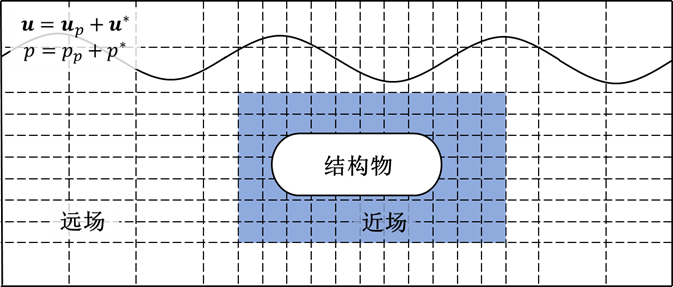
\includegraphics[width=0.6\textwidth]{figures/ch1-Helmholtz-示意图.png}
	\caption{Helmholtz速度分解示意图}
	\label{fig:ch1-Helmholtz-示意图}
\end{myfigure}
\begin{myfigure}
	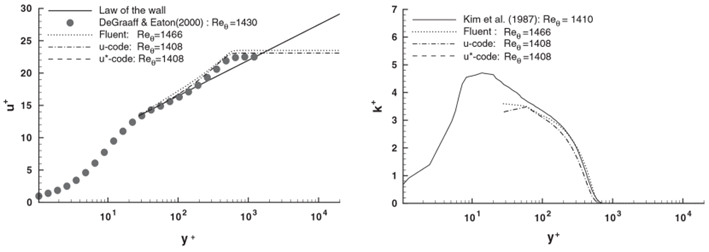
\includegraphics[width=0.9\textwidth]{figures/ch1-Helmholtz-Kim.png}
	\caption{二维平板流平均流向速度(左)和湍流动能(右)\cite{kimComplementaryRANSEquations2005}：耦合方法、全粘流方法和试验结果对比}
	\label{fig:ch1-Helmholtz-Kim}
\end{myfigure}

Hafez等人\cite{hafezImprovedNumericalSimulations2007}通过修正Bernoulli方程求得势流压力，并将其代入粘流方程求解。%
使用该方法分别对中等雷诺数不可压条件下，定常和非定常的二维翼型绕流进行了计算，结果与全粘流方法吻合较好。%
上海交通大学的赵骥、朱仁传等人\cite{ZhaoChuanBoShuiDongLiDeNianShiLiuOuHeFangFaChuTan2015,%
ZhaoJiYuHelmholtzSuDuFenJieDeNianShiLiuOuHeFangFa2016,%
ZhaoQiuJieSUBOFFRaoLiuWenTiDeNianShiLiuOuHeFangFa2017}使用该方法实现了二维圆柱绕流模拟，%
并在此基础上推广至三维，实现了三维潜体绕流的耦合计算。%
并且使用该方法计算了Wigley船的航行阻力，其中兴波阻力通过势流方法求解，而粘性阻力使用势粘流耦合方法求解获得，计算结果与试验和文献数据吻合较好。

Edmund等人\cite{edmundVelocityDecompositionMethod2012}同样将整场速度分解为势流项和互补项，并对粘流域进行了截断，势流域为粘流域提供边界条件。%
但势流模型需要求解包含物面边界的Laplace方程，并通过迭代计算以满足势粘流解的收敛性和一致性。%
研究中对二维翼型绕流、圆柱绕流以及三维潜体湍流进行了模拟，与全粘流方法和试验结果吻合良好，%
并且实现了粘流计算域的缩减，部分结果如\cref{fig:ch1-Helmholtz-Edmund}所示。%
Rosemurgy等人\cite{rosemurgyVelocityDecompositionApproach2012}将该方法推广到定常自由表面流动，%
并通过模拟流过池底凸起结构的定常自由面流验证了其有效性。%
Chen等人\cite{chenVelocityDecompositionApproach2015}发展了这种方法的非定常自由表面流动形式，%
并将其进一步推广到三维并应用于Wigley船型的湍流模拟，相较于全粘流方法提高了近50\%的计算效率。
\begin{myfigure}
	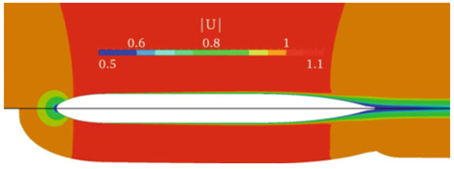
\includegraphics[width=0.6\textwidth]{figures/ch1-Helmholtz-Edmund.png}
	\caption{二维潜体湍流速度场\cite{edmundVelocitydecompositionFormulationIncompressible2013}：全粘流方法(上)和耦合方法(下)对比}
	\label{fig:ch1-Helmholtz-Edmund}
\end{myfigure}

Zhang\cite{zhangMultimodelMethodSimulating2018}采用了类似Kim等人\cite{kimComplementaryRANSEquations2005}的方法对速度进行分解，%
并通过两相流Euler求解器求解势流部分。%
值得注意的是，流固耦合问题在势流域中也需要求解，并且绕射波、辐射波等由欧拉方程求解。%
势流解通过松弛区域单向传递至粘流域，在这点上该方法与区域分解方法有相似之处。%
在他们的研究中，对复杂海底地形下的二维波浪结构物作用问题进行了模拟，与全粘流方法和试验结果基本一致，并且计算耗时能够节省50\%甚至85\%。

由互补NS方程求得的互补项中所包含的粘性效应，如果在实际计算中不加以处理，其衰减并不快。同时，在耦合计算中所有的粘流离散点都需要赋予势流解，因此对计算成本的减小并不显著。而Edmund\cite{edmundVelocityDecompositionMethod2012,edmundImprovedViscousInviscid2011,%
edmundVelocitydecompositionFormulationIncompressible2013}的方法虽然对粘流域进行了截断，但需要进行迭代运算，%
因此相比于Kim等\cite{kimComplementaryRANSEquations2005}的方法计算量更大。%
此外，在面对如波浪破碎等复杂的两相流问题时，进行速度分解是有困难的，因此Helmholtz速度分解法暂时只被用于较为简单问题的势粘流耦合研究。%

船舶和海洋工程相比其他领域而言，自由液面的存在是其一大突出特点，并且对自由液面的模拟增加了数值计算成本。%
基于此，研究人员提出了SWENSE模型。SWENSE模型最初由Ferrant等人\cite{ferrantNewRANSEPotential2002,ferrantPotentialRANSEApproach2003}提出，%
其基本思想是将速度、压力和自由面高度等分解为入射项和其他剩余项，如\cref{fig:ch1-SWENSE-示意图}所示。其表达如下：
\begin{equation}
	\bm{u} = \bm{u}_{\rm{I}} + \bm{u}_{\rm{D}},\quad %
	\bm{p} = \bm{p}_{\rm{I}} + \bm{p}_{\rm{D}},\quad %
	\bm{\eta} = \bm{\eta}_{\rm{I}} + \bm{\eta}_{\rm{D}}
\end{equation}
并推导得到修正的NS方程：
\begin{equation}
	\frac{\partial \bm{u}_{\rm{D}}}{\partial t} +\left(\bm{u}\cdot\nabla\right)\bm{u}_{\rm{D}} %
	- \nu\nabla^2\bm{u}_{\rm{D}} + \frac{\nabla p_{\rm{D}}}{\rho} %
	= - \left(\bm{u}_{\rm{D}}\cdot\nabla\right)\bm{u}_{\rm{I}} + \nu\nabla^2\bm{u}_{\rm{I}}
\end{equation}
式中$\nu$为运动粘性系数。二维情况下，质量守恒方程和运动学、动力学自由面条件为：
\begin{subequations}
	\begin{gather}
	\nabla\cdot\bm{u} = 0 \\ % 
	\frac{\partial \eta_{\rm{D}}}{\partial t} %
	+ \left(\bm{u}_{\rm{D}}\cdot\bm{i}\right)\left(\nabla\eta_{\rm{I}}\cdot\bm{i}\right) %
	+ \left(\bm{u}\cdot\bm{i}\right)\left(\nabla\eta_{\rm{D}}\cdot\bm{i}\right) %
	= \bm{u}_{\rm{D}}\cdot\bm{j} \\ % 不编号
	p_{\rm{D}} = \rho\bm{g}\eta_{\rm{D}} + 2\rho\nu\left(\nabla\cdot\bm{n}\right)\left(\bm{u}\cdot\bm{n}\right) \\ %
	\left(\bm{n}\cdot\nabla\right)\left(\bm{u}\cdot\bm{\tau}\right) %
	+ \left(\bm{\tau}\cdot\nabla\right)\left(\bm{u}\cdot\bm{n}\right) = 0 %
	\end{gather}
\end{subequations}
以上这一组方程即为SWENSE方程组。%
式中：$\bm{i}$、$\bm{j}$分别为水平和竖直方向的方向向量，$\bm{\tau}$和$\bm{n}$分别为自由液面处的切向和法向。%
SWENSE方程求解过程中，入射项由势流方法求解给出，而剩余项由SWENSE粘流求解器获得。%
在求解过程中，每一时间步内先由势流方法求解给出入射波，然后粘流求解器根据入射波求解辐射、绕射和粘性流动等问题。%
这是一种基于方程分解的单向耦合，粘流模型对势流没有反馈。
\begin{myfigure}
	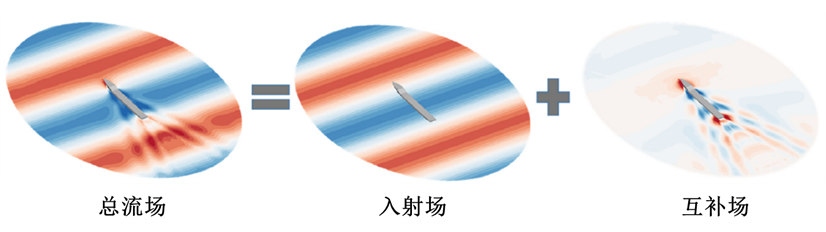
\includegraphics[width=0.8\textwidth]{figures/ch1-SWENSE-示意图.png}
	\caption{SWENSE模型示意图\cite{yuNumericalStudyWavestructure2022a}}
	\label{fig:ch1-SWENSE-示意图}
\end{myfigure}

Luquet等人\cite{luquetApplicationSWENSEMethod2007,luquetSimulationTLPWaves2007}%
和Alessandrini等人\cite{alessandriniNumericalSimulationShip2008}通过HOS方法给出入射波，%
对Wigley船在规则波中的二自由度运动以及固定半潜式平台在聚焦波中的载荷响应进行了全尺度模拟。%
Wigley船的垂荡和纵摇运动以及平台的载荷计算结果均与试验一致。%
Monroy等人\cite{monroyRANSSimulationsShip2009}使用该方法计算了重吊船在规则波和不规则波迎浪工况下的垂荡和纵摇响应，%
并进行了模型试验，其结果进一步验证了此数值方法的准确性。

早期的SWENSE模型未采用自由面捕捉技术，在解决自由面大变形、波浪破碎等复杂的两相流问题上较为困难。%
Reliquet等人\cite{reliquetSimulationWaveBodyInteraction2013,reliquetSimulationsDelft3722019}采用交错网格布置，配合LSM方法实现了两相流求解。%
采用该方法对静水和迎浪中船舶的模拟结果\cite{reliquetSimulationWaveBodyInteraction2013}与试验结果对比良好，%
如\cref{fig:ch1-SWENSE-Reliquet}所示。%
对不同傅汝德数下的双体船进行耐波性计算\cite{reliquetSimulationsDelft3722019}，其结果与全粘流方法以及试验结果吻合较好。%
进一步地，Vukčević\cite{vukcevicNumericalModellingCoupled2016}针对扰动波反射问题，在SWENSE求解器中添加了隐式松弛区域。%
类似地，他们的研究中也采用了LSM方法对自由面进行捕捉，模拟了二维数值水池和竖直圆柱的高阶波浪力。%
其数值结果与试验和文献结果吻合良好，并对计算中的波浪条件、离散条件等进行了分析。%
Gatin等人\cite{gatinFrameworkEfficientIrregular2017}采用Vukčević\cite{vukcevicNumericalModellingCoupled2016}的方法%
模拟了三维实尺度集装箱船遭遇极端波浪。%
在此工况下，船体出现了大幅横荡和横摇运动，并且捕捉到了上浪现象。%
除了LSM方法以外，Li等人\cite{liCalculationHighorderWave2017,liProgressCouplingPotential2018}将VOF方法引入SWENSE模型以实现两相流求解。%
通过对二维数值水池以及规则波中竖直圆柱的计算，验证了该方法的有效性和准确性，如\cref{fig:ch1-SWENSE-Li}所示。%
此外，Li等人\cite{liSpectralWaveExplicit2021}还模拟了规则波、不规则波工况下的固定CALM浮标模型，%
与全粘流方法和试验结果对比显示，在相同网格数下耦合方法精度好于全粘流方法，而在相同精度要求下其计算效率也高于后者。%
\begin{myfigure}
	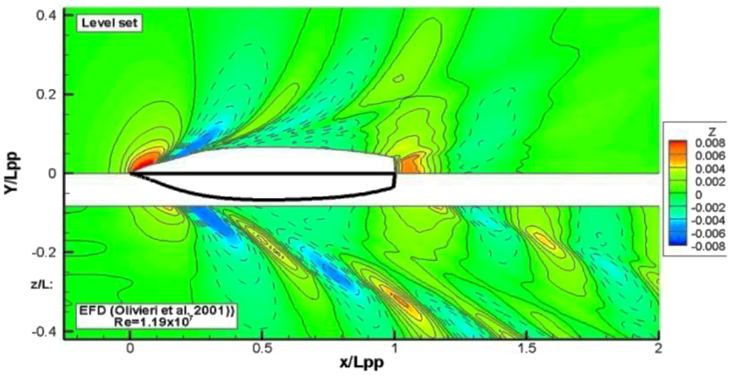
\includegraphics[width=0.6\textwidth]{figures/ch1-SWENSE-Reliquet.png}
	\caption{船体近场自由面高\cite{reliquetSimulationWaveBodyInteraction2013}：耦合方法(上半)与试验结果(下半)对比}
	\label{fig:ch1-SWENSE-Reliquet}
\end{myfigure}
\begin{myfigure}
	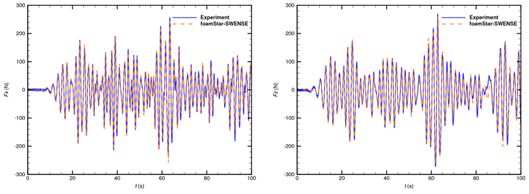
\includegraphics[width=0.8\textwidth]{figures/ch1-SWENSE-Li.png}
	\caption{CALM浮标波浪载荷\cite{liCalculationHighorderWave2017}：水平波浪力(左)和竖直波浪力(右)，耦合方法与试验结果对比}
	\label{fig:ch1-SWENSE-Li}
\end{myfigure}

SWENSE模型是目前较为成熟的势粘流耦合方程分解方法。%
由于SWENSE边界无需施加入射波条件，因此能够有效地降低方程组边界条件的复杂度，在保证精度的前提下提高计算速度。%
并且经过不断发展，该方法能够解决的问题类型也越来越丰富。%
但是SWENSE求解器的开发和优化难度较大，并且面对不合适求解的问题时修改的灵活性较差。

方程分解方法的研究进展总结如\cref{tab:ch1-FD-progress}所示。%
方程分解方法从流动控制方程中解耦出势流部分，采用势流方法对其独立求解，再将势流部分代入互补NS方程的求解以实现耦合。%
Helmholtz速度分解方法将流动分解为势流项和剩余项，因此辐射、绕射等问题一般由势流求解，而粘性、湍流等由互补NS方程求解。%
而SWENSE模型将流动分解为入射项和剩余项，其中入射项通过势流求解给出，因此辐射、绕射以及粘性和湍流等问题均由SWENSE求解器解得。%
\begin{mylongtable}
	{M{1.8cm} M{4.5cm} M{2cm} M{7.5cm}}
	{方程分解方法研究进展}
	{tab:ch1-FD-progress}
	{\toprule
		{分解模型} & {研究人员} & {自由面技术} & {应用问题} \\
		\midrule
	}
	{\multicolumn{4}{c}{\cref{tab:ch1-FD-progress} 方程分解方法研究进展(续表)} \\
		\toprule
		{分解模型} & {研究人员} & {自由面技术} & {应用问题} \\
		\midrule
	}
	{\bottomrule}
	{\bottomrule}
	& {Kim等\cite{kimComplementaryRANSEquations2005} (2005)} & {——} & {平板流、方形管道流、机翼绕流 (2D)} \\
	& {Hafez等\cite{hamiltonViscousInviscidMatching2011} (2007)} & {——} & {机翼绕流 (2D)} \\
	\multirow{2}{1.8cm}{\centering Helmoholtz速度分解} %
	& {Edmund等\cite{edmundVelocitydecompositionFormulationIncompressible2013} (2013)} & {——} & {二维翼型和圆柱绕流、潜体湍流 (2D、3D)} \\
	& {Rosemurgy等\cite{rosemurgyVelocityDecompositionApproach2012} (2012)} & {——} & {流过池底凸起结构的定常自由面流 (2D)} \\
	& {Chen等\cite{chenVelocityDecompositionApproach2015} (2015)} & {——} & {有限长平板层流、Wigley船湍流 (3D)} \\
	& {Zhang\cite{zhangMultimodelMethodSimulating2018} (2018)} & {VOF} & {复杂海底地形波浪结构物作用 (2D)} \\
	\hline
	& {Ferrant\cite{ferrantNewRANSEPotential2002,ferrantPotentialRANSEApproach2003} (2003)} & {——} & {规则波与固定方形潜体作用 (2D)} \\
	& \makecell{Luquet等\cite{luquetApplicationSWENSEMethod2007,luquetSimulationTLPWaves2007} (2007) \\ %
	Alessandrini等\cite{alessandriniNumericalSimulationShip2008}(2008)} & {——} & {Wigley船二自由度运动、聚焦波与固定半潜式平台作用 (3D)} \\
	& {Gentaz\cite{gentazNumericalSimulation3D2008} (2008)} & {——} & {波浪中的竖直圆柱 (3D)} \\
	& {Monroy等\cite{monroyRANSSimulationsShip2009} (2009)} & {——} & {重吊船在波浪中的二自由度响应 (3D)} \\
	\multirow{2}{1.8cm}{\centering SWENSE模型} %
	& {Reliquet等\cite{reliquetSimulationWaveBodyInteraction2013} (2013)} & {LSM} & {静水和迎浪中的船舶 (3D)} \\
	& {Reliquet等\cite{reliquetSimulationsDelft3722019} (2019)} & {LSM} & {不同傅汝德数下双体船的耐波性 (3D)} \\
	& {Vukčević等\cite{vukcevicNumericalModellingCoupled2016} (2016)} & {LSM} & {数值水池、竖直圆柱高阶波浪力 (2D、3D)} \\
	& {Gatin等人\cite{gatinFrameworkEfficientIrregular2017} (2017)} & {LSM} & {实尺度集装箱船遭遇极端波浪 (3D)} \\
	& {Li等\cite{liCalculationHighorderWave2017,liProgressCouplingPotential2018,liSpectralWaveExplicit2021} (2021)} %
	& {VOF} & {二维数值水池、规则波中的竖直圆柱、不同工况下的固定CALM浮标模型 (2D、3D)} \\
	& {Aliyar\cite{aliyarExtremeWaveInteraction2022} (2022)} & {VOF} & {圆柱波浪爬升、浮式风机波固耦合 (3D)} \\
	& {Yu等\cite{yuNumericalStudyWavestructure2022a} (2022)} & {LSM} & {有/无航速典型船舶在波浪中的动力响应 (3D)} \\
\end{mylongtable}

方程分解方法对船舶耐波性、波浪力计算等问题的解决比较成熟，%
在保持精度的前提下能够有效提高计算效率，甚至在同等计算资源条件下能够提高求解精度。%
虽然方程分解方法在两相流问题的解决上已经有很大进步，但是面对自由面大变形甚至波浪破碎等复杂问题时求解仍然困难。

\subsection{
  \texorpdfstring{本文研究内容及特点} % 正文和目录中显示的标题
  {\thesubsection 本文研究内容及特点} % 书签页中显示的标题
}
\label{ssec:本文研究内容及特点}

综上所述，恶劣海况下波浪与浮式平台强非线性作用这一多尺度问题的CFD方法数值模拟仍具有一些缺陷。%
第一，CFD方法在模拟大尺度极端波浪演化时具有严重的数值耗散和色散；%
第二，CFD方法在同时模拟大尺度波浪演化、主尺度平台运动以及小尺度砰击作用这一多尺度问题时，对计算资源的需求十分巨大并且是工程上难以接受的；%
第三，传统有网格CFD方法在模拟砰击这一类自由液面大变形问题时，需要在自由液面处布置大量精细网格以准确捕捉液面变化，这会带来更严重的计算消耗。%

因此本文尝试探索一种基于无网格CFD方法的势粘流耦合模型，将浮式平台遭受波浪强非线性作用这一多尺度问题进行分解并实现多模型耦合求解，%
以实现在保证计算精度的前提下尽量减少计算资源消耗。%
目前势粘流耦合方法研究主要集中于船舶耐波性操纵性、数值水池造波等问题，而针对波浪与结构物强非线性相互作用问题的研究较少。%
并且大多数势粘流耦合研究中所采用的CFD方法为有网格方法，而基于无网格CFD方法的势粘流耦合研究相对较少，耦合模型的计算精度和效率仍待提升。%

本文将采用区域分解方法进行基于无网格CFD方法的势粘流耦合模型开发，主要有以下几点原因：%
(1)区域分解方法和方程分解方法对自由液面不发生大变形的问题进行模拟时，二者的计算精度和效率相近\cite{robauxAssessmentOnewayCoupling2022}，%
但区域分解方法不需要修改NS控制方程，其开发和优化相对更为容易；%
(2)方程分解方法对于自由液面发生大变形、翻卷甚至破碎等问题的模拟较为复杂，对自由液面处的处理比较困难；%
(3)本文所采用的无网格CFD方法目前还不适合采用方程分解方法进行势粘流耦合。%

基于区域分解方法，波浪与浮式平台强非线性作用这一多尺度问题可以分解为大尺度波浪演化、主尺度平台运动和小尺度强非线性作用。%
在势粘流耦合模型中，大尺度波浪演化通过势流方法求解，而主尺度平台运动和小尺度砰击作用通过无网格CFD方法求解。%
这样一来既能够提高波浪模拟的质量，又能够有效地降低计算资源消耗，从而提高数值模拟的准确性和效率。%
本文将结合势流方法能够快速准确地模拟波浪的优势以及CFD方法能够模拟强非线性自由液面运动问题的能力，%
初步探索面向波浪与浮式平台强非线性作用问题的势粘流耦合方法，并在二维上实现数值算法开发。本文的主要工作内容如下：

(1)	基于高阶谱开源求解器HOS-NWT与改进的光滑粒子流体动力学$\delta^+$-SPH模型，构建HOS-SPH势粘流单向耦合模型，%
以实现通过HOS方法为SPH方法提供入射波边界条件，从而提高波浪模拟质量和计算效率；

(2)	基于有限水深二维时域Rankine源边界元法，在HOS-SPH势粘流单向耦合模型的基础上进行HOS-SPH-BEM势粘流多模型耦合算法开发，%
以实现势粘流间流场信息的双向传递，从而进一步提高数值计算精度；

(3)	对势粘流耦合算法进行验证和测试，主要考察对计算精度和效率的提高。

本文框架如\cref{fig:ch1-论文框架图}所示：
\begin{myfigure}
	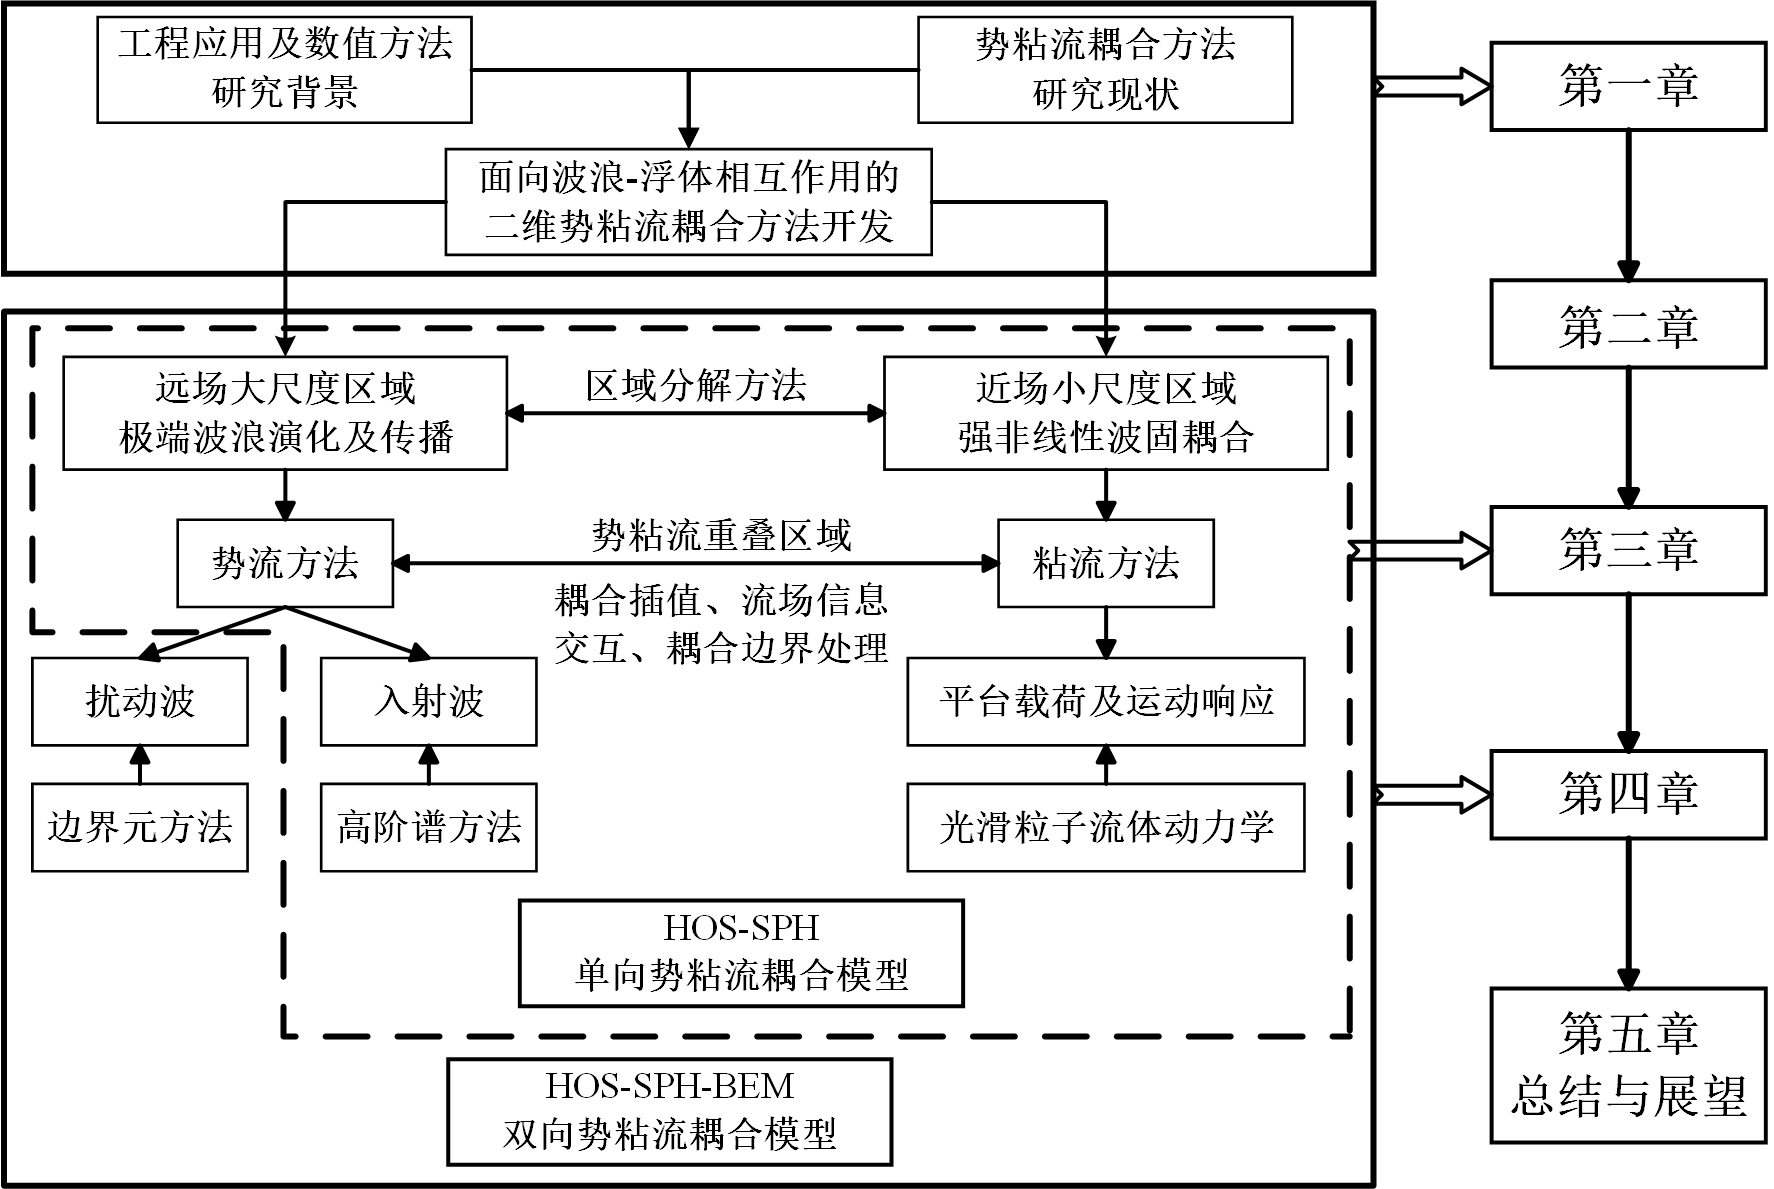
\includegraphics[width=0.99\textwidth]{figures/ch1-论文框架图.png}
	\caption{论文框架图}
	\label{fig:ch1-论文框架图}
\end{myfigure}

本文共分为五个章节，具体安排如下：%
第1章介绍选题背景与研究意义和势粘流耦合方法研究现状；%
第2章介绍所使用的数值方法和求解器，并通过数值波浪模拟对它们进行验证；%
第3章在HOS方法和SPH方法的基础上构建HOS-SPH势粘流单向耦合模型，并通过数值算例对HOS-SPH单向耦合方法进行验证和分析；%
第4章建立基于BEM方法和SPH方法的SPH-BEM势粘流双向耦合方法，并实现基于该方法的数值消波。%
而后在HOS-SPH单向耦合方法和SPH-BEM双向耦合方法的基础上进一步构建HOS-SPH-BEM势粘流多模型耦合方法，并对其进行验证；%
最后对全文的工作进行总结和展望。
% 第2章 数值方法介绍
\newoddpage % 创建新的奇数页
\section{
  \texorpdfstring{数值方法介绍} % 正文和目录中显示的标题
  {\thesection 数值方法介绍} % 书签页中显示的标题
}
\label{sec:数值方法介绍}

目前船舶与海洋工程领域的势粘流耦合方法研究主要集中于非线性波浪数值模拟、极端波浪演化与传播和船舶耐波性与操纵性等问题，%
而对于砰击、上浪等涉及强非线性自由液面现象的问题研究较少。%
因此本文针对海上浮式平台遭受波浪砰击、上浪等强非线性自由液面运动问题，%
基于非线性势流高阶谱方法、边界元方法以及无网格光滑粒子流体动力学方法开展势粘流耦合方法的研究。%

本章首先分别介绍几种势粘流数值方法的基本理论和所采用的求解器，包括：%
高阶谱方法的基本理论以及所采用的开源求解器HOS-NWT数值水池，%
二维时域Rankine源边界元方法以及基于该方法所实现的数值水池，%
光滑粒子流体动力学方法和改进的$\delta^+$-SPH模型。%
最后通过规则波和不规则波的数值波浪模拟分析了几种方法的收敛性和准确性，并对不同方法结果进行了对比。

\subsection{
  \texorpdfstring{高阶谱方法} % 正文和目录中显示的标题
  {\thesubsection 高阶谱方法} % 书签页中显示的标题
}
\label{ssec:高阶谱方法}

\subsubsection{
  \texorpdfstring{高阶谱方法基础理论} % 正文和目录中显示的标题
  {\thesubsubsection 高阶谱方法基础理论} % 书签页中显示的标题
}
\label{sssec:高阶谱方法基础理论}

高阶谱方法(High Order Spectral，简称HOS)是一种基于势流理论的伪谱方法，%
最早由Dommermuth和Yue\cite{dommermuthHighorderSpectralMethod1987a}以及%
West等人\cite{westNewNumericalMethod1987a}分别提出。%
在HOS方法中，流体满足无粘不可压以及无旋流假设，并且波陡符合小量假设。%
流动通过速度势$\phi\left(\bm{x},z,t\right)$进行描述，其满足Laplace方程、自由液面运动学和动力学条件：
\begin{equation}
  \nabla^2\phi\left(\bm{x},z,t\right) = 0
  \label{eq:HOS-Laplace}
\end{equation}
\begin{equation}
  \frac{\partial \eta}{\partial t} + \frac{\partial \phi}{\partial \bm{x}}\frac{\partial \eta}{\partial \bm{x}} %
  - \frac{\partial \phi}{\partial z} = 0,\quad z = \eta
  \label{eq:HOS-KFBC}
\end{equation}
\begin{equation}
  \frac{\partial \phi}{\partial t} %
  + \frac{1}2 \left[\left(\frac{\partial \phi}{\partial \bm{x}}\right)^2 %
  + \frac{\partial \phi}{\partial z}^2\right] + g\eta = 0,\quad z = \eta
  \label{eq:HOS-DFBC}
\end{equation}
式中：$\eta = \left(\bm{x},t\right)$为波高，$g$为重力加速度。%
$\bm{x} = \left(x,y\right)$为水平方向位置向量(二维情况下不考虑$y$方向)，$z$为竖直方向坐标，$t$为时间。

根据Zakharov方程\cite{zakharovStabilityPeriodicWaves1968}，将自由面上的速度势定义为：
\begin{equation}
  \phi^s\left(\bm{x},t\right) = \phi\left[\bm{x},\eta\left(\bm{x},t\right),t\right]
  \label{eq:HOS-Zakharov}
\end{equation}

将\cref{eq:HOS-Zakharov}带入\cref{eq:HOS-KFBC}和\cref{eq:HOS-DFBC}中可得关于$\phi^s$和$\eta$的边界控制方程：
\begin{equation}
  \frac{\partial \eta}{\partial t} + \frac{\partial\phi^s}{\partial \bm{x}}\frac{\partial\eta}{\partial \bm{x}} %
  - \left(1 + \frac{\partial\eta}{\partial \bm{x}}\frac{\partial\eta}{\partial \bm{x}}\right)%
  \frac{\partial\phi^s}{\partial z} = 0,\quad z = \eta
  \label{eq:HOS-BCE-phi}
\end{equation}
\begin{equation}
  \frac{\partial\phi^s}{\partial t} + g\eta %
  + \frac{1}2\frac{\partial\phi^s}{\partial\bm{x}}\frac{\partial\phi^s}{\partial\bm{x}} %
  - \frac{1}2\left(1 + \frac{\partial\eta}{\partial \bm{x}}\frac{\partial\eta}{\partial \bm{x}}\right) %
  \left(\frac{\partial\phi^s}{\partial z}\right)^2 = 0,\quad z = \eta
  \label{eq:HOS-BCE-eta}
\end{equation}

假设$\phi$和$\eta$为$O\left(\epsilon\right)$阶小量，并将速度势以波陡为小量进行$M$阶摄动展开得到：
\begin{equation}
  \phi\left(\bm{x},z,t\right) = \sum_{m=1}^{M}\phi^{\left(m\right)}\left(\bm{x},z,t\right)
  \label{eq:HOS-perturbation}
\end{equation}

而后将摄动展开的每一项$\phi^{\left(m\right)}$进行泰勒展开，并代入\cref{eq:HOS-perturbation}得到：
\begin{equation}
  \phi^s\left(\bm{x},t\right) = \phi\left(\bm{x},\eta,t\right) %
  = \sum_{m=1}^{M}\sum_{k=0}^{M-m}\frac{\eta^k}{k!}\frac{\partial^k}{\partial z^k} %
  \phi^{\left(m\right)}\left(\bm{x},0,t\right)
  \label{eq:HOS-Taylor}
\end{equation}

将\cref{eq:HOS-Taylor}展开并合并同阶项，整理可得到$\phi^{\left(m\right)}$在平均水面处的边界条件方程：
\begin{eqnarray}
  \phi^{\left(m\right)}\left(\bm{x},0,t\right) = R^{\left(m\right)}, \quad m = 1, 2, 3, \cdots, M
\end{eqnarray}
其中：
\begin{subequations}
  \begin{gather}
    R^{\left(1\right)} = \phi^s \\
    R^{\left(m\right)} = - \sum_{k=1}^{m-1}\frac{\eta^k}{k!}\frac{\partial^k}{\partial z^k}\phi^{m-k}\left(\bm{x},0,t\right), %
    \quad m = 1, 2, 3, \cdots, M
  \end{gather}
\end{subequations}
通过给定的初始自由液面边界条件$\phi^s$和$\eta$，可以依上式递推得出摄动展开的各阶项$\phi^{\left(m\right)}$。

在HOS方法中，空间导数的求解在傅里叶频域空间进行，而一般变量的求解在物理空间进行。%
为了实现这点，将摄动展开的各阶项$\phi^{\left(m\right)}$进行模态展开得到：
\begin{equation}
  \phi^{\left(m\right)}\left(\bm{x},z,t\right) = \sum_{n=0}^{m}\phi_n^{\left(m\right)}\left(t\right) %
  \psi_n\left(\bm{x},z\right)
  \label{eq:HOS-modes}
\end{equation}
其中$\psi_n\left(\bm{x},z\right)$为满足Laplace方程和各边界条件的基函数。%
对于无限水深和有限水深问题分别取不同的基函数：

无限水深：
\begin{equation}
  \phi^{\left(m\right)}\left(\bm{x},z,t\right) = \sum_{n=0}^{m} \phi_n^{\left(m\right)}\left(t\right) %
  \exp\left[\left|\bm{k}_n\right|z + i\bm{k}_n\cdot \bm{x}\right]
\end{equation}

有限水深：
\begin{equation}
  \phi^{\left(m\right)}\left(\bm{x},z,t\right) = \sum_{n=0}^{m} \phi_n^{\left(m\right)}\left(t\right) %
  \frac{\cosh\left[\left|\bm{k}_n\right|\left(z + h\right)\right]}{\cosh\left(\left|\bm{k}_n\right|h\right)}%
  \exp\left(i\bm{k}_n\cdot \bm{x}\right)
\end{equation}
式中：$\bm{k}_n = \left(k_x,k_y\right)$为波数向量，$\left|\bm{k}_n\right| = \sqrt{{k_x}^2 + {k_y}^2}$，%
$k_x = 2\pi i/L_x$，$k_y = 2\pi i/L_y$，其中$i$、$j$、$L_x$、$L_y$分别表示$x$、 $y$方向上的模态数和长度%
(二维情况下不考虑$y$方向)，在数值计算中会对模态数进行截断。

将\cref{eq:HOS-modes}带入\cref{eq:HOS-Taylor}并给出自由面速度势在$z$方向上的导数：
\begin{equation}
  \phi_z\left(\bm{x},\eta,t\right) = \sum_{m=1}^{M}\sum_{k=0}^{M-m}\frac{\eta^k}{k!}%
  \sum_{n=1}^{N} \phi_n^{\left(m\right)}\left(t\right) \frac{\partial^{k+1}}{\partial z^{k+1}}%
  \psi_n\left(\bm{x},0\right)
  \label{eq:HOS-derivative-z}
\end{equation}
其中$\phi_n^{\left(m\right)}\left(t\right)$可以通过%
对$\phi^{\left(m\right)}$进行快速傅里叶变换(Fast Fourier Transform，简称FFT)得到，%
从而实现在傅里叶频域空间对速度势空间导数进行求解。

将\cref{eq:HOS-derivative-z}带入自由液面边界条件\cref{eq:HOS-BCE-phi}和%
\cref{eq:HOS-BCE-eta}可得关于$\phi^s$和$\eta$的方程：
\begin{subequations}
  \begin{gather}
    \frac{\partial n}{\partial t} %
    + \left(\frac{\partial\phi^s}{\partial\bm{x}} \frac{\partial\eta}{\partial\bm{x}}\right) %
    \left[\sum_{m=1}^{M}\sum_{k=0}^{M-m}\frac{\eta^k}{k!}%
    \sum_{n=1}^{N} \phi_n^{\left(m\right)}\left(t\right) \frac{\partial^{k+1}}{\partial z^{k+1}}%
    \psi_n\left(\bm{x},0\right)\right] = 0 %
    \label{eq:HOS-ODE-phi} \\
    %
    \frac{\partial\phi^s}{\partial t} + g\eta %
    + \frac{1}2\frac{\partial\phi^s}{\partial\bm{x}}\frac{\partial\phi^s}{\partial\bm{x}} %
    - \frac{1}2\left(1 + \frac{\partial\eta}{\partial \bm{x}}\frac{\partial\eta}{\partial \bm{x}}\right) %
    \left[\sum_{m=1}^{M}\sum_{k=0}^{M-m}\frac{\eta^k}{k!}%
    \sum_{n=1}^{N} \phi_n^{\left(m\right)}\left(t\right) \frac{\partial^{k+1}}{\partial z^{k+1}}%
    \psi_n\left(\bm{x},0\right)\right]^2 = 0 %
    \label{eq:HOS-ODE-eta}
  \end{gather}
\end{subequations}

当给定初始自由液面边界条件$\phi^s$和$\eta$时，%
通过对\cref{eq:HOS-ODE-phi}和\cref{eq:HOS-ODE-eta}进行积分可以实现时间上的步进。%
由于HOS方法在数值计算过程中引入了FFT方法，因此该数值方法是伪谱法，%
并且具有较高的计算效率和精度\cite{seiffertSimulationBreakingWaves2018}

\subsubsection{
  \texorpdfstring{HOS-NWT数值水池} % 正文和目录中显示的标题
  {\thesubsubsection HOS-NWT数值水池} % 书签页中显示的标题
}
\label{sssec:HOS-NWT数值水池}

本文所采用的HOS求解器是法国南特中央理工大学的Ducrozet等人发布的%
开源数值水池HOS-NWT\cite{ducrozetModifiedHighOrderSpectral2012}，%
该求解器能够实现最高达到三阶非线性的数值造波，其基本理论可见\cref{sssec:高阶谱方法基础理论}所述。%
在数值水池造波过程中，需要考虑造波机运动所产生的造波边界条件和消波区域的设置，如\cref{fig:ch2-HOS-NWT}所示。%
\begin{myfigure}
  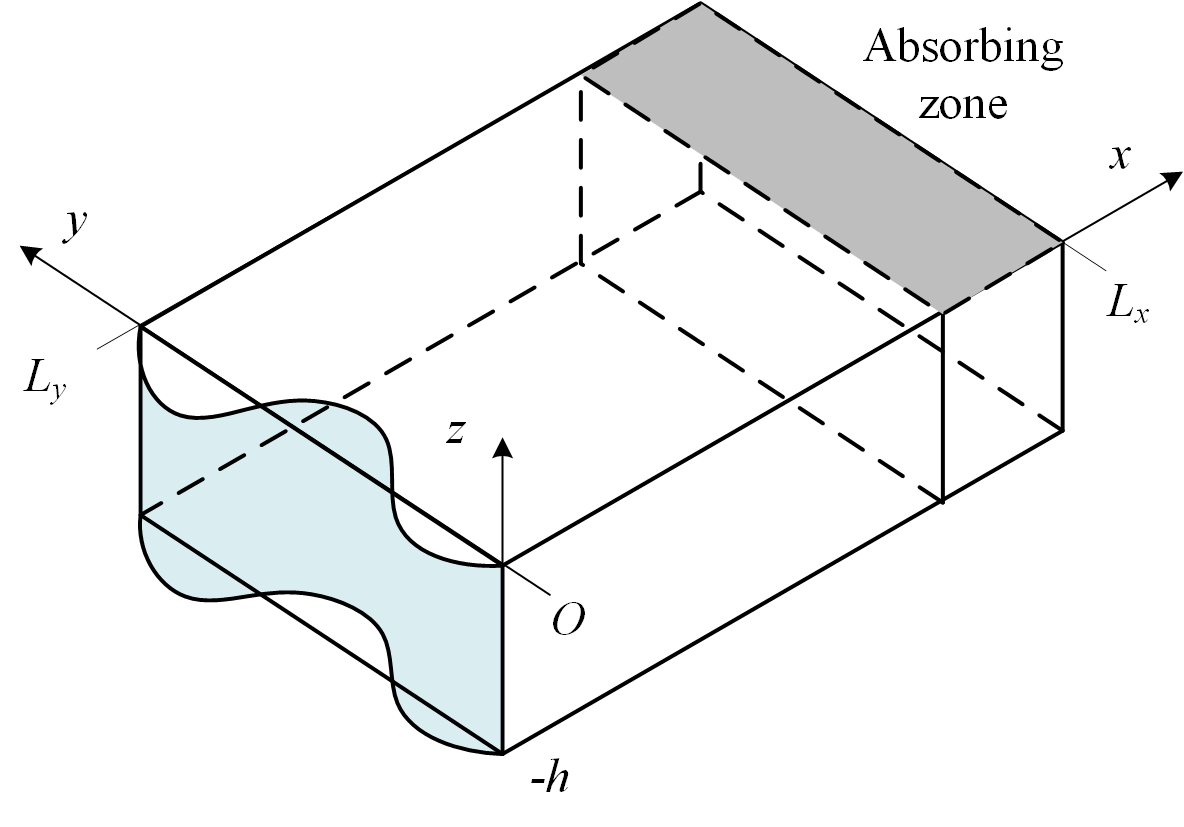
\includegraphics[width=0.5\textwidth]{figures/ch2-HOS-NWT.png}
  \caption{HOS-NWT数值水池方案及其坐标系}
  \label{fig:ch2-HOS-NWT}
\end{myfigure}

其中消波区域$\Omega_{\rm{Absorbing}}$是通过对自由液面上的压力进行局部修正来实现的，%
修正压力为\cite{bonnefoyFullyspectral3DTimedomain2006}：
\begin{equation}
  p^{*} = \rho\nu\left(x\right) \frac{\partial\phi}{\partial\bm{x}} \cdot \bm{n}, \quad z = \eta
\end{equation}
式中：$\nu\left(x\right)$为修正函数，$\bm{n}$为自由液面的法向量。

下面简单介绍在HOS-NWT数值水池中造波边界条件的处理。

将造波机的运动描述为壁面在$x$方向上的运动$X = X\left(y,z,t\right)$(二维情况下不考虑$y$方向)，则造波边界条件可以表达为：
\begin{equation}
  \frac{\partial X}{\partial t} = \frac{\partial\phi}{\partial x} %
  - \nabla_{yz}X \cdot \nabla_{yz}\phi, x = X\left(y,z,t\right)
\end{equation}
式中：$\nabla_{yz} = \left(\dfrac{\partial}{\partial y}, \dfrac{\partial}{\partial z}\right)$。

HOS-NWT通过引入附加速度势处理该造波边界条件，将总速度势分解为两个分量$\phi = \phi_{\rm{spec}} + \phi_{\rm{add}}$。%
其中$\phi_{\rm{spec}}$为描述固定壁面水池(即$X = 0$时)自由液面演化的速度势，%
而$\phi_{\rm{add}}$为考虑造波边界条件的附加速度势。 %
除了需要满足Laplace方程和壁面边界条件外，还需要满足造波边界条件。%
将自由面上的速度势$\phi_{\rm{spec}}$定义为$\phi^s\left(\bm{x},t\right) = \phi_{\rm{spec}}\left(\bm{x},\eta,t\right)$，%
则自由液面边界条件\cref{eq:HOS-BCE-phi}和\cref{eq:HOS-BCE-eta}由于$\phi_{\rm{add}}$的引入被改写为：
\begin{equation}
  \left\{
    \begin{aligned}
    \frac{\partial\eta}{\partial t} =& %
    \left(1 + \frac{\partial\eta}{\partial \bm{x}}\frac{\partial\eta}{\partial \bm{x}}\right) %
    \frac{\partial\phi^s}{\partial z} %
    - \frac{\partial\left(\phi^s + \phi_{\rm{add}}\right)}{\partial\bm{x}} \frac{\partial\eta}{\partial\bm{x}} %
    + \frac{\partial\phi_{\rm{add}}}{\partial z} \\
    %
    \frac{\partial\phi^s}{\partial t} =& - g\eta %
    - \frac{1}2 \frac{\partial\phi^s}{\partial\bm{x}} \frac{\partial\phi^s}{\partial\bm{x}} %
    + \frac{1}2\left(1 + \frac{\partial\eta}{\partial \bm{x}}\frac{\partial\eta}{\partial \bm{x}}\right) %
    \left(\frac{\partial\phi^s}{\partial z}\right)^2 \\
    &- \frac{\partial\phi^s}{\partial\bm{x}} \frac{\partial\phi_{\rm{add}}}{\partial\bm{x}} %
    - \frac{1}2 \frac{\partial\phi_{\rm{add}}}{\partial\bm{x}}\frac{\partial\phi_{\rm{add}}}{\partial\bm{x}} %
    - \frac{\partial\phi_{\rm{add}}}{\partial t} - \nu \frac{\partial\eta}{\partial t}
    \end{aligned}
  \right. %
  , \quad z = \eta
  \label{eq:HOS-NWT-FBC}
\end{equation}

因此$\phi_{\rm{spec}}$和$\phi_{\rm{add}}$分别满足下列的边界条件：
\begin{equation}
  \left\{
    \begin{aligned}
      & \nabla^2\phi_{\rm{spec}} = 0, \quad \left(x,y,z\right) \in \Omega \\
      %
      & \frac{\partial \phi_{\rm{spec}}}{\partial n} = 0, \quad x = 0, L_x; y = 0; z = -h \\
      %
      & \text{引入}\phi_{\rm{add}}\text{的自由液面边界条件}, \text{即\cref{eq:HOS-NWT-FBC}}, %
      \quad z = \eta\left(\bm{x},t\right)
    \end{aligned}
  \right. 
  \label{eq:HOS-NWT-BC-spec}
\end{equation}
\begin{equation}
  \left\{
    \begin{aligned}
      & \nabla^2\phi_{\rm{add}} = 0, \quad \left(x,y,z\right) \in \Omega \\
      %
      & \frac{\partial \phi_{\rm{add}}}{\partial n} = \quad x = 0, L_x; y = 0; z = -h \\
      %
      & \frac{\partial \phi_{\rm{add}}}{\partial X} + \nabla_{yz}X \cdot \nabla_{yz}\phi_{\rm{add}} = %
      \frac{\partial X}{\partial t} \frac{\phi_{\rm{spec}}}{\partial X} %
      - \nabla_{yz}X \cdot \nabla_{yz}\phi_{\rm{spec}}, \quad x = X\left(y,z,t\right)
    \end{aligned}
  \right. 
  \label{eq:HOS-NWT-BC-add}
\end{equation}

根据\cref{eq:HOS-NWT-BC-spec}和\cref{eq:HOS-NWT-BC-add}，数值波浪模拟被分解为两个问题。%
首先求解出满足造波边界条件的附加速度势$\phi_{\rm{add}}$，%
而后根据改写的自由液面边界条件\cref{eq:HOS-NWT-FBC}求解$\phi_{\rm{spec}}$，从而实现整个问题的求解。%

HOS-NWT中采用SWEET模型\cite{bonnefoyFullyspectral3DTimedomain2006,bonnefoyFullyspectral3DTimedomain2006a}%
对附加速度势进行求解，%
并且Guillaume等人\cite{ducrozetModifiedHighOrderSpectral2012} 将该模型的造波边界条件推广到了三阶非线性。%
计算中采用自适应步长的四阶Runge–Kutta Cash–Karp时间推进格式\cite{cashVariableOrderRungeKutta1990}。%

在所发布的HOS-NWT求解器中，计算的初始条件为波浪信息，%
如规则波的周期和波高、不规则波的波浪谱等，其中还内置了JONSWAP波浪谱可以用于计算使用。%
为了便于与试验或其他数值方进行对比，本文在HOS-NWT求解器的基础上，%
添加了以造波机运动作为边界条件的功能，从而能够根据造波机的运动时程实现数值造波。

\subsection{
  \texorpdfstring{边界元方法} % 正文和目录中显示的标题
  {\thesubsection 边界元方法} % 书签页中显示的标题
}
\label{ssec:边界元方法}

边界元方法(Boundary Element Method，简称BEM)是十分成熟的势流方法。%
本文参考文献\parencite{grilliNumericalModelingWave1996,SunErWeiZiYouMianTiaoJianHeFuSheTiaoJianDeShuZhiMoNi2004}%
实现了基于二维时域Rankine源边界元法的数值波浪水池，下面简单介绍边界元方法的基础理论。

\subsubsection{
  \texorpdfstring{边界积分方程} % 正文和目录中显示的标题
  {\thesubsubsection 边界积分方程} % 书签页中显示的标题
}
\label{sssec:边界积分方程}

在无粘、不可压以及无旋流假设下，流动可以通过速度势$\phi$进行描述，%
控制方程为Laplace方程\cref{eq:HOS-Laplace}，通过格林第三公式可以将其转换为边界积分方程：
\begin{equation}
  \alpha\left(P\right) \phi\left(P,t\right) %
  + \int_{\Gamma} \left[\phi\left(Q,t\right) \frac{\partial G_{PQ}}{\partial n_Q} %
  - \frac{\partial \phi\left(Q,t\right)}{\partial n_Q}G_{PQ}\right] {\rm{d}} l = 0
  \label{eq:BEM-BIE}
\end{equation}
其中$G$为二维Rankine源格林函数：
\begin{equation}
  \left\{
    \begin{aligned}
      & G_{PQ} = G\left(P,Q\right) = \ln\frac{1}{\bm{r}_{PQ}} %
      = \ln \frac{1}{\sqrt{\left(x_P - x_Q\right)^2 + \left(z_P - z_Q\right)^2}} \\
      % 
      & \frac{\partial G_{PQ}}{\partial n_Q} = -\frac{\left(\bm{r}_Q - \bm{r}_P\right)}{{r_{PQ}}^2} \cdot n_Q
    \end{aligned}
  \right.
\end{equation}
式中：$P$，$Q$分别表示流场中的场点和边界上的源点，$r$为位置矢量，$n$为流场边界的外法向。%
$\alpha\left(P\right)$为场点处的空间角，当$P$位于流场内部，$\alpha\left(P\right) = 2\pi$；%
当$P$位于流场边界，$\alpha\left(P\right)$为边界在该点的张开角。%
对于直线、一阶或高阶光滑曲线等连续边界，$\alpha\left(P\right) = \pi$。

对于二维有限水深的数值波浪水池，需要考虑造波机边界$\Gamma_w$、固壁边界$\Gamma_s$和自由液面边界$\Gamma_f$这三种边界。%
其中造波机边界$\Gamma_w$和固壁边界$\Gamma_s$的边界条件为Newmann边界条件，而自由液面边界$\Gamma_f$为Dirichlet边界条件。%
因此根据各个边界上所提供的边界条件不同，离散的边界积分方程可以分别写为：
\begin{subequations}
  \begin{align}
    \begin{aligned}
      \alpha_i\phi_i + \sum_{P_j\in \Gamma_w\cap\Gamma_s}\phi_j %
      \int_{\Delta\Gamma} \frac{\partial G_{ij}}{\partial n_j} {\rm{d}} l %
      - \sum_{P_j\in \Gamma_f}\frac{\partial \phi_j}{\partial n_j} %
      \int_{\Delta\Gamma} G_{ij} {\rm{d}} l =& \\%
      \sum_{P_j\in \Gamma_w\cap\Gamma_s}\frac{\partial \phi_j}{\partial n_j} %
      \int_{\Delta\Gamma} G_{ij} {\rm{d}} l %
      - \sum_{P_j\in \Gamma_f}\phi_j & %
      \int_{\Delta\Gamma} \frac{\partial G_{ij}}{\partial n_j} {\rm{d}} l %
    \end{aligned}, \quad & P_i \in \Gamma_w \cap \Gamma_s
    \label{eq:BEM-discrete-BIE-1} \\
    %
    \begin{aligned}
      \sum_{P_j\in \Gamma_w\cap\Gamma_s}\phi_j %
      \int_{\Delta\Gamma} \frac{\partial G_{ij}}{\partial n_j} {\rm{d}} l %
      - \sum_{P_j\in \Gamma_f}\frac{\partial \phi_j}{\partial n_j} %
      \int_{\Delta\Gamma} G_{ij} {\rm{d}} l =& \\%
      \alpha_i\phi_i + \sum_{P_j\in \Gamma_w\cap\Gamma_s}\frac{\partial \phi_j}{\partial n_j} %
      \int_{\Delta\Gamma} G_{ij} {\rm{d}} l %
      -& \sum_{P_j\in \Gamma_f}\phi_j %
      \int_{\Delta\Gamma} \frac{\partial G_{ij}}{\partial n_j} {\rm{d}} l %
    \end{aligned}, \quad & P_i \in \Gamma_f
    \label{eq:BEM-discrete-BIE-2}
  \end{align}
\end{subequations}
式中：下标i和j表示边界离散单元的编号。经过整理\cref{eq:BEM-discrete-BIE-1}和\cref{eq:BEM-discrete-BIE-2}可写为矩阵形式：
\begin{equation}
  \begin{bmatrix}
    H^1 & H^2
  \end{bmatrix}
  \begin{bmatrix}
    \phi^N \\ \dfrac{\partial \phi^D}{\partial n}
  \end{bmatrix}
  = 
  \begin{bmatrix}
    G^1 & G^2
  \end{bmatrix}
  \begin{bmatrix}
    \dfrac{\partial \phi^N}{\partial n} \\ \phi^D
  \end{bmatrix}
  \label{eq:BEM-BIE-matrix}
\end{equation}
其中：
\begin{subequations}
  \begin{align}
    & \left\{
      \begin{aligned}
        & H_{ij}^1 = \alpha_i \delta_{ij} + \int_{\Delta\Gamma} \frac{\partial G_{ij}}{\partial n_j} {\rm{d}} l \\
        & G_{ij}^1 = \int_{\Delta\Gamma} G_{ij} {\rm{d}} l
      \end{aligned}
    \right.
    , \quad P_i \in \Gamma_w \cap \Gamma_s \\
    %
    & \left\{
      \begin{aligned}
        & H_{ij}^2 = - \int_{\Delta\Gamma} G_{ij} {\rm{d}} l \\
        & G_{ij}^1 = - \alpha_i \delta_{ij} - \int_{\Delta\Gamma} \frac{\partial G_{ij}}{\partial n_j} {\rm{d}} l
      \end{aligned}
    \right.
    , \quad P_i \in \Gamma_f
  \end{align}
\end{subequations}
式中：上标$N$和$D$分别表示Newmann边界条件和Dirichlet边界条件的边界处。%
由于本文所采用的为线性自由液面边界条件，各个边界均为直线，因此点源和点偶的积分可以解析求解。%
但当$i = j$时源偶积分具有奇异性，%
因此本文参考文献\parencite{ZangYueLongGuanYuBianJieYuanFaZhongQiYiJiFenDeChuLi1994}中%对奇异积分的处理方式进行求解。

\subsubsection{
  \texorpdfstring{边界条件} % 正文和目录中显示的标题
  {\thesubsubsection 边界条件} % 书签页中显示的标题
}
\label{sssec:BEM-边界条件}

求解\cref{eq:BEM-BIE-matrix}中的边界积分方程需要提供流场边界上的边界条件，下面分别介绍各个边界上边界条件的求解方式。

造波机边界和固壁边界上所提供的为Newmann边界条件。以活塞式造波机为例，造波机边界和固壁边界上的边界条件可以分别表示为：
\begin{equation}
  \frac{\partial\phi}{\partial n} = 
  \left\{
    \begin{aligned}
      \bm{u}_w \cdot \bm{n}, \quad & \bm{r} \in \Gamma_w \\
      0, \quad & \bm{r} \in \Gamma_s
    \end{aligned}
  \right.
  \label{eq:BEM-WBC}
\end{equation}
式中：$\bm{u}_w$为造波机的速度，在计算时只需提供造波机的运动即可。

线性自由液面边界条件为：
\begin{equation}
  \frac{\partial^2\phi}{\partial t^2} + g \frac{\partial \phi}{\partial z} = 0, \quad z = 0
  \label{eq:BEM-FBC}
\end{equation}

为了避免波浪在水池末端的固壁上发生反射，本文采取在自由液面边界条件中添加Rayleigh阻尼的方式对其进行消波。%
修改后的自由液面边界条件可以写为：
\begin{equation}
  \frac{\partial^2\phi}{\partial t^2} + \chi \frac{\partial\phi}{\partial t} %
  + g \frac{\partial \phi}{\partial z} = 0, \quad z = 0
  \label{eq:BEM-FBC-modified}
\end{equation}
其中阻尼$\chi$的取值为：
\begin{equation}
  \chi = 
  \left\{
    \begin{aligned}
      & \chi_0 \frac{\left|x - x_{\rm{Absorbing}}\right|}{L_{\rm{Absorbing}}}, \quad & \bm{r} \in \Gamma_{\rm{Absorbing}} \\
      & 0, \quad & \bm{r} \notin \Gamma_{\rm{Absorbing}}
    \end{aligned}
  \right.
\end{equation}
式中：$\chi_0$为阻尼系数，在本文计算中均取为$\chi_0 = 5.0$。%
参考文献\parencite{SunErWeiZiYouMianTiaoJianHeFuSheTiaoJianDeShuZhiMoNi2004}%
对\cref{eq:BEM-FBC-modified}进行离散可以获得离散格式的自由液面边界条件：
\begin{equation}
  \phi\left(\bm{r},t_n\right) = \phi\left(0\right) %
  + n \Delta t \frac{\partial\phi\left(\bm{r},0\right)}{\partial t} %
  - \mu \Delta t \sum_{m=0}^{n-1}\phi\left(\bm{r},t_m\right) %
  - g {\Delta t}^2 \left[\sum_{m=1}^{n-1}\left(n - m\right) %
  \frac{\partial \phi\left(\bm{r},t_m\right)}{\partial \eta} %
  + \frac{n}2 \frac{\partial \phi\left(\bm{r},0\right)}{\partial \eta}\right]
  \label{eq:BEM-FBC-discrete}
\end{equation}
式中：$t_n = n \Delta t$。在完成上一时间步的边界积分方程求解后，%
根据\cref{eq:BEM-FBC-discrete}可以求出下一时间步自由液面上的$\phi$，即Dirichlet边界条件。

在进行每一时间步的求解时，只需根据\cref{eq:BEM-WBC}和\cref{eq:BEM-FBC-discrete}求出各个边界上的边界条件，%
然后代入\cref{eq:BEM-BIE-matrix}对边界积分方程进行求解，从而可以实现整个问题的求解。%
计算中时间步长的取值符合CFL条件，即$\Delta t = {\rm{CFL}} \cdot \Delta x$，%
本文中BEM计算的CFL数参考文献\parencite{SunErWeiZiYouMianTiaoJianHeFuSheTiaoJianDeShuZhiMoNi2004}中取为${\rm{CFL}} = 1/\sqrt{gd}$。

\subsection{
  \texorpdfstring{光滑粒子流体动力学方法} % 正文和目录中显示的标题
  {\thesubsection 光滑粒子流体动力学方法} % 书签页中显示的标题
}
\label{ssec:光滑粒子流体动力学方法}

光滑粒子流体动力学方法(Smoothed Particle Hydrodynamics，简称SPH)是一种无网格拉格朗日粒子法。%
在弱可压SPH方法中，压力基于状态方程通过密度进行求解\cite{monaghanSimulatingFreeSurface1994}，因此该方法是显式推进的。%
早期的SPH方法在求解压力场时有较为严重的波动，Marrone等人\cite{marroneDSPHModelSimulating2011}所提出的%
$\delta$-SPH模型通过在控制方程中引入密度耗散项和人工粘性项较好地解决了这一问题。%
Sun等人\cite{sunDplusSPHModelSimple2017,sunInclusionAcousticDamper2023}%
所提出的$\delta^+$-SPH模型在$\delta$-SPH模型的基础上，%
通过粒子位移修正技术和声阻尼技术进一步提高了压力场求解的精度，本文所采用的即为$\delta^+$-SPH模型。

\subsubsection{
  \texorpdfstring{控制方程} % 正文和目录中显示的标题
  {\thesubsubsection 控制方程} % 书签页中显示的标题
}
\label{sssec:SPH-控制方程}

SPH方法的基本控制方程为：
\begin{equation}
  \left\{
    \begin{aligned}
      & \frac{{\rm{D}}\rho}{{\rm{D}}t} = - \rho \nabla \cdot \bm{u} \\
      & \frac{{\rm{D}}\bm{u}}{{\rm{D}}t} = \frac{\nabla \cdot \bm{T}}{\rho} + \bm{g} \\
      & \frac{{\rm{D}}\bm{r}}{{\rm{D}}t} = \bm{u} \\
      & p = p\left(\rho\right)
    \end{aligned}
  \right.
  \label{eq:SPH-CE}
\end{equation}
式中：${\rm{D}}/{\rm{D}}t$表示随体导数，%
$\rho$、$\bm{u}$和$\bm{r}$分别表示流体微团的密度、速度矢量和位置矢量，%
$\bm{g}$为重力加速度，$\bm{T}$为流体的应力张量。%
由于在一般的海洋工程水动力问题中，流体的可压缩性在计算时是可忽略的，%
从而不考虑体积粘性产生的影响，因此$\nabla \cdot \bm{T}$可以展开为：
\begin{equation}
  \nabla \cdot \bm{T} = - \nabla p + \mu \nabla^2 \bm{u}
\end{equation}
式中：$p$为流体微团的各向同性压力，$\mu$为流体的动力粘性系数。

在求解水动力问题时，\cref{eq:SPH-CE}中的压力状态方程常采用简化的Tait状态方程\cite{antuonoFreesurfaceFlowsSolved2010}：
\begin{equation}
  p \approx {c_0}^2 \left(\rho - \rho_0\right)
\end{equation}
式中：$c_0$为人工声速，$\rho_0$为参考密度(即$p = 0$时的流体密度)。%
为了满足弱可压假设，人工声速$c_0$的选择需要满足以下条件\cite{antuonoEnergyBalanceDSPH2015}：
\begin{equation}
  c_0 \ge 10 \max \left(U_{\max}, \sqrt{\frac{p_{\max}}\rho_0}\right)
\end{equation}
式中：$U_{\max}$和$p_{\max}$分别为预估的流场最大速度和压力。

\subsubsection{
  \texorpdfstring{核近似和粒子近似} % 正文和目录中显示的标题
  {\thesubsubsection 核近似和粒子近似} % 书签页中显示的标题
}
\label{sssec:核近似和粒子近似}

在SPH方法中，流体被离散为均匀分布的粒子而非网格，%
并且流体的物理属性被赋予在粒子上，这一离散过程由核近似和粒子近似这两个部分组成。%

核近似理论中，一般量的物理场$f\left(\bm{r}\right)$及其导数通过卷积积分进行插值：
\begin{equation}
  \left\{
    \begin{aligned}
      & f\left(\bm{r}\right) \approx \left\langle f\left(\bm{r}\right)\right\rangle %
      = \int_{\Omega} f\left(\bm{r}^{*}\right) W\left(\bm{r} - \bm{r}^{*}; h\right) {\rm{d}} \bm{r}^{*} \\
      %
      & \nabla_{\bm{r}} f\left(\bm{r}\right) \approx \left\langle \nabla_{\bm{r}} f\left(\bm{r}\right)\right\rangle %
      = \int_{\Omega} f\left(\bm{r}^{*}\right) \nabla_{\bm{r}} W\left(\bm{r} - \bm{r}^{*}; h\right) {\rm{d}} \bm{r}^{*} 
    \end{aligned}
  \right.
\end{equation}
式中：$\bm{r}$为一般的空间点坐标， $\nabla_{\bm{r}}$表示相对位置$\bm{r}$的梯度，%
$\left\langle f\left(\bm{r}\right)\right\rangle$被称为$f\left(\bm{r}\right)$的核近似。%
$W\left(\bm{r} - \bm{r}^{*}; h\right)$为权重函数，也称为核函数，%
其中$h$为紧支域$\Omega$的特征长度，也称为光滑长度。%
核函数需要满足对称性条件和归一性条件，以及狄拉克函数性质等\cite{liuSmoothedParticleHydrodynamics2003}，即：
\begin{subequations}
  \begin{gather}
    W\left( \bm{r}-{\bm{r}^{*}};h \right) %
    = W\left( {\bm{r}^{*}}-\bm{r};h \right) \label{eq:SPH-kernel-symmetry}\\ 
    \int_{\Omega}{W\left( \bm{r}-{\bm{r}^{*}};h \right)%
    {\rm{d}}{\bm{r}^{*}}} = 1 \label{eq:SPH-kernel-normalization} \\ 
    \lim_{h \to 0} W\left( \bm{r}-{\bm{r}^{*}};h \right) %
    = \delta \left( \bm{r}-{\bm{r}^{*}} \right) \label{eq:SPH-kernel-dirac}
  \end{gather} 
\end{subequations}

本文所采用的核函数为Wendland的C2核函数\cite{wendlandPiecewisePolynomialPositive1995}，在二维情况下其表达式为：
\begin{equation}
  W\left( \bm{r}-{\bm{r}^{*}};h \right) %
  = \frac{7}{\pi {{h}_{s}}^2}{{\left( 1-\frac{\left| \bm{r}-{\bm{r}^{*}} \right|}{{{h}_{s}}} \right)}^{4}} %
  \left( 1+4\frac{\left| \bm{r}-{\bm{r}^{*}} \right|}{{{h}_{s}}} \right)
\end{equation}

式中：$h_s = k_s h$，其中$k_s = 2.0$。%
该核函数相比传统的高阶样条函数更加便于计算，并且具有更好的数值收敛性\cite{dehnenImprovingConvergenceSmoothed2012}。

根据\cref{eq:SPH-kernel-normalization}，核函数导数满足%
$\int_{\Omega}{\nabla_{\bm{r}}W\left( \bm{r}-{\bm{r}^{*}};h \right){\rm{d}}{\bm{r}^{*}}} = 0$，%
因此$\left\langle \nabla_{\bm{r}} f\left(\bm{r}\right)\right\rangle$和%
$\left\langle \nabla_{\bm{r}} \cdot f\left(\bm{r}\right)\right\rangle$分别可以写为如下不同的离散形式：
\begin{subequations}
  \begin{align}
    & \left\langle \nabla_{\bm{r}} f\left(\bm{r}\right)\right\rangle = %
    \int_{\Omega} \left[f\left(\bm{r}^{*}\right) - f\left(\bm{r}\right)\right] %
    \nabla_{\bm{r}} W\left(\bm{r} - \bm{r}^{*}; h\right) {\rm{d}} \bm{r}^{*} \label{eq:SPH-kernel-gradient-1}\\
    & \left\langle \nabla_{\bm{r}} f\left(\bm{r}\right)\right\rangle = %
    \int_{\Omega} \left[f\left(\bm{r}^{*}\right) + f\left(\bm{r}\right)\right] %
    \nabla_{\bm{r}} W\left(\bm{r} - \bm{r}^{*}; h\right) {\rm{d}} \bm{r}^{*} \label{eq:SPH-kernel-gradient-2} \\
    & \left\langle \nabla_{\bm{r}} \cdot f\left(\bm{r}\right)\right\rangle = %
    \int_{\Omega} \left[f\left(\bm{r}^{*}\right) - f\left(\bm{r}\right)\right] \cdot %
    \nabla_{\bm{r}} W\left(\bm{r} - \bm{r}^{*}; h\right) {\rm{d}} \bm{r}^{*} \label{eq:SPH-kernel-divergence-1}\\
    & \left\langle \nabla_{\bm{r}} \cdot f\left(\bm{r}\right)\right\rangle = %
    \int_{\Omega} \left[f\left(\bm{r}^{*}\right) + f\left(\bm{r}\right)\right] \cdot %
    \nabla_{\bm{r}} W\left(\bm{r} - \bm{r}^{*}; h\right) {\rm{d}} \bm{r}^{*} \label{eq:SPH-kernel-divergence-2}
  \end{align}
\end{subequations}

\cref{eq:SPH-kernel-gradient-2}由于具有更好的守恒性，常被用于离散动量方程中的压力梯度项；%
而\cref{eq:SPH-kernel-divergence-1}由于在自由液面处核函数被截断时具有更好的一致性，%
常被用于离散连续性方程中的速度散度项\cite{colagrossiTheoreticalConsiderationsFreesurface2009}。

粒子近似，即为将核近似中的连续积分离散为基于粒子的求和计算。%
根据核近似的结果，常用的粒子近似离散公式有：
\begin{equation}
  \left\{
    \begin{aligned}
      & f\left(\bm{r}_i\right) = \sum_j f\left(\bm{r}_j\right) W_{ij} V_j \\
      & \nabla_i f\left(\bm{r}_i\right) = \sum_j %
      \left[f\left(\bm{r}_j\right) + f\left(\bm{r}_i\right)\right] \nabla_i W_{ij} V_j \\
      & \nabla_i \cdot f\left(\bm{r}_i\right) = \sum_j %
      \left[f\left(\bm{r}_j\right) + f\left(\bm{r}_i\right)\right] \cdot \nabla_i W_{ij} V_j \\
    \end{aligned}
  \right.
\end{equation}
式中：下标$i$和$j$为粒子编号，求和运算时$j$为粒子$i$的紧支域$\Omega$内的所有粒子。%
$\nabla_i$为对粒子$i$的空间导数，$V_i = m_i/\rho_i$为粒子体积，其中$m$为粒子的质量。%
$W_{ij} = W\left(\bm{r}_i - \bm{r}_j; h\right)$为核函数的简写。%
由于粒子近似的特点，积分运算被离散为基于粒子的求和运算，并且状态方程的引入使得控制方程能够显式求解，%
因此SPH方法的程序结构十分适合于并行计算，大大提高了该方法的计算效率。

\subsubsection{
  \texorpdfstring{$\delta^+$-SPH模型的离散控制方程} % 正文和目录中显示的标题
  {\thesubsubsection delta-plus-SPH模型的离散控制方程} % 书签页中显示的标题
}
\label{sssec:Delta-plus-SPH模型的离散控制方程}

采用SPH方法的离散方式对控制方程进行离散，即可得到离散化的控制方程。%
在$\delta^+$-SPH模型中，离散化的控制方程如下：
\begin{equation}
  \left\{ 
    \begin{aligned}
      & \frac{{\rm{D}}\rho_i}{{\rm{D}}t} = %
      - \rho_i\sum_j\left( \bm{u}_j-\bm{u}_i \right)\cdot {\nabla_i}W_{ij}V_j+D_i^\rho \\ 
      & \frac{{\rm{D}}\bm{u}_i}{{\rm{D}}t} =%
       - \frac{1}{\rho_i}\sum_j\left(p_j + p_i\right){\nabla_i}W_{ij}V_j+\bm{g}+\pi_i^{\nu }+\lambda_i^{ad} \\ 
      & \frac{{\rm{D}}\bm{r}_i}{{\rm{D}}t} = \bm{u}_i; %
      \quad \bm{r}_i\to \left( \bm{r}_i+\delta \bm{r}_i \right) \\ 
      & p_i = {c_0}^2\left( \rho_i-\rho_0 \right) \\  
    \end{aligned}
  \right.
  \label{eq:DSPH-discrete}
\end{equation}
\cref{eq:DSPH-discrete}中在\cref{sssec:SPH-控制方程}和\cref{sssec:核近似和粒子近似}内介绍过的符号不再赘述。%
下面详细介绍控制方程中各个修正项的作用以及在本文计算中各项参数的选择。
\begin{equation}
  \left\{
    \begin{aligned}
      & D_i^\rho=\delta h{c_0}{{D}_i};%
      \qquad {{D}_i} = 2\sum_j\psi_{ij} %
      \frac{\left( \bm{r}_j-\bm{r}_i \right)\cdot {\nabla_i}W_{ij}V_j}%
      {{{\left| \bm{r}_j-\bm{r}_i \right|}^2}} \\ 
      & \psi_{ij} = \left( \rho_j - \rho_i \right) %
      - 0.5\left[ \left\langle \nabla \rho \right\rangle _i^{L} %
      + \left\langle \nabla \rho \right\rangle _j^{L} \right]\cdot \left( \bm{r}_j-\bm{r}_i \right) \\ 
      & \pi_i^{\nu }=\alpha h{c_0}\frac{\rho_0}{\rho_i}\sum_j\pi_{ij}{\nabla_i}W_{ij}V_j; %
      \qquad {\pi_{ij}}=\frac{\left( \bm{u}_j-\bm{u}_i \right)\cdot \left( \bm{r}_j-\bm{r}_i \right)} %
      {{{\left| \bm{r}_j-\bm{r}_i \right|}^2}} \\ 
      & \lambda_i^{ad} = {{\alpha }_2}h{c_0}\frac{\rho_0}{\rho_i} %
      \sum_j\left( {{\lambda }_i}+{{\lambda }_j} \right){\nabla_i}W_{ij}V_j; %
      \qquad {{\lambda }_i}=\sum_j\left( \bm{u}_j-\bm{u}_i \right)\cdot {\nabla_i}W_{ij}V_j \\ 
      & \delta \bm{r}_i = - {\rm{CFL}}\cdot Ma\cdot {{\left( 2h \right)}^2}\cdot %
      \sum_j\left[ 1+R{{\left( \frac{W_{ij}}{W\left( \Delta x \right)} \right)}^{n}} \right] %
      {\nabla_i}W_{ij}\frac{m_j}{\left( \rho_i+\rho_j \right)}
    \end{aligned}
  \right.
\end{equation}

在计算过程中光滑长度为$h = \alpha_s\Delta x$，%
其中$\Delta x$为初始的粒子间距，而$\alpha_s$为光滑系数，决定了紧支域内的粒子数量，%
由于本文中的计算均为二维问题，因此该参数取为$\alpha_s = 2.0$\cite{zhangSmoothedParticleHydrodynamics2017}。

在\cref{sssec:SPH-控制方程}中提到人工声速$c_0$需要满足一定条件，%
针对本文所涉及的数值水池问题，其选取主要与水池深度有关，%
在计算中取为$c_0 = 10\sqrt{gd}$，其中$d$为水池深度。

$D_i^{\rho}$为人工扩散项\cite{molteniSimpleProcedureImprove2009}，也称为密度耗散项，%
能够有效解决计算过程中流场内部出现的高频压力振荡。%
其中的$\left\langle \nabla\rho \right\rangle ^L$为采用修正的粒子近似方法进行离散的重整化密度梯度，%
因此能够确保在自由液面处核函数截断的情况下，密度梯度的计算仍具有二阶精度\cite{randlesSmoothedParticleHydrodynamics1996}。%
$\delta$是与问题无关的参数，在本文计算中参考文献\parencite{antuonoNumericalDiffusiveTerms2012}取为$\delta = 0.1$。%

$\pi_i^{\nu}$为人工粘性项\cite{marroneDSPHModelSimulating2011}，%
能够提高数值计算稳定性，并且可以一定程度上使流场粒子的分布更加均匀。%
但是由于过高的人工粘性会导致计算结果的失真，因此在本文的计算中如非特殊说明，%
人工粘性系数$\alpha$参考文献\parencite{antuonoNumericalDiffusiveTerms2012}均取为$\alpha = 0.02$。%

$\lambda_i^{ad}$为声阻尼项\cite{sunInclusionAcousticDamper2023}，%
能够有效地去除在计算中由于弱可压假设而产生的非物理声波，%
因此能够从压力场中去除由于该声波而造成的压力振荡，从而进一步提高压力场的计算精度。%
计算中声阻尼系数$\alpha_2$越大则对声波产生的抑制效果越强，%
但是过大的$\alpha_2$会使结果失真，并且会影响时间步长的选取，%
因此本文计算中参考文献\parencite{sunInclusionAcousticDamper2023}选取为$\alpha_2 = 1.0$。


Sun等人\cite{sunDplusSPHModelSimple2017}提出了一项基于弱可压假设建立的粒子位移修正技术 %
(Particle Shifting Technique，简称PST)。%
该技术在速度更新位移的基础上对粒子位移进行额外修正，以确保计算中粒子的均匀分布。%
其中$\delta\bm{r}_i$为位移的额外修正量，CFL为库朗数(Courant-Friedrichs-Lewy constant，简称CFL)，%
$Ma = U_{\max}$为流动马赫数，其中$U_{\max}$为流场中的最大速度。%
$R$和$n$为常数，本文计算中参考文献\parencite{monaghanSPHTensileInstability2000}分别取为$R = 0.2$和$n = 4$。

\subsubsection{
  \texorpdfstring{边界条件} % 正文和目录中显示的标题
  {\thesubsubsection 边界条件} % 书签页中显示的标题
}
\label{sssec:SPH-边界条件}

本文所涉及问题的SPH流场示意图如\cref{fig:ch2-SPH-field}所示，其中包括自由液面边界$\Gamma_{\rm{Free-surface}}$，%
固壁边界$\Gamma_{\rm{Wall}}$和流入流出边界$\Gamma_{\rm{Inflow}}$/$\Gamma_{\rm{Outflow}}$。%
下面简单介绍各类边界条件及其处理方式\cite{SunWuTiYuZiYouYeMianOuHeZuoYongDeGuangHuaLiZiLiuTiDongLiXueFangFaYanJiu2018}。
\begin{myfigure}
  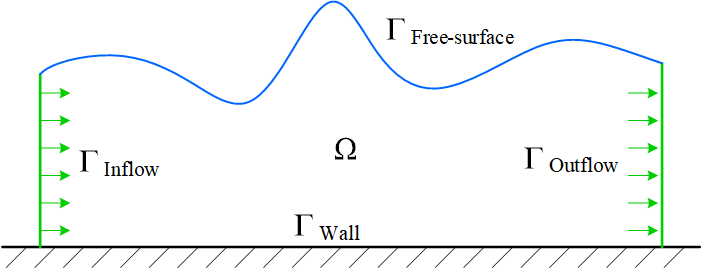
\includegraphics[width=0.6\textwidth]{figures/ch2-SPH-field.png}
  \caption{SPH流场示意图}
  \label{fig:ch2-SPH-field}
\end{myfigure}

(1)	自由液面边界条件

自由液面运动学边界条件要求初始时刻在自由液面处的流体微团在液面不发生破碎的情况下仍保持在自由液面上，%
即自由液面处流体微团的法向速度与自由液面的法向速度相等：
\begin{equation}
  \bm{u} \cdot \bm{n}_{\Gamma_{\rm{Free-surface}}} %
  = \bm{u}_{\Gamma_{\rm{Free-surface}}} \cdot \bm{n}_{\Gamma_{\rm{Free-surface}}}, %
  \quad \bm{r} \in \Gamma_{\rm{Free-surface}}
\end{equation}
式中：$\bm{u}$和$\bm{u}_{\Gamma_{\rm{Free-surface}}}$分别为流体微团和自由液面的速度，%
$\bm{n}_{\Gamma_{\rm{Free-surface}}}$为自由液面的外法向。

自由液面动力学边界条件在不考虑表面张力时，要求在跨越自由表面时的压力连续。%
在本文中不考虑气相的影响，因此可以认为自由液面处的压力为$p = 0$。%
由于在SPH方法中压力通过状态方程求解，因此自由液面处的密度为$\rho = \rho_0$。%
从而动力学边界条件可以写为：
\begin{equation}
  \nabla \cdot \bm{u} = -\frac{1}{\rho} \frac{{\rm{D}}\rho}{{\rm{D}}t} = 0, %
  \quad \bm{r} \in \Gamma_{\rm{Free-surface}}
\end{equation}

由于SPH方法是拉格朗日方法，因此自由液面运动学边界条件能够被隐式满足。%
而对于弱可压SPH方法，如果采用合适的离散格式\cite{colagrossiTheoreticalConsiderationsFreesurface2009}，%
自由液面动力学边界条件也可以被隐式满足。%
因此在$\delta^+$-SPH模型中无需额外处理即可隐式满足自由液面边界条件，这也是该方法适合于模拟自由液面流动的主要原因之一。

(2)	固壁边界条件%

固壁边界处首先需要满足无穿透条件，并且根据是否考虑壁面的粘性力作用可以分为无滑移和自由滑移这两种边界条件。%
由于在本文所涉及的波浪与结构物相互作用问题中，流体对结构物的粘性力作用远小于压力作用，%
因此可以忽略壁面粘性作用而采用自由滑移边界条件：
\begin{equation}
  \bm{u} \cdot \bm{n}_{\Gamma_{\rm{Wall}}} %
  = \bm{u}_{\Gamma_{\rm{Wall}}} \cdot \bm{n}_{\Gamma_{\rm{Wall}}}, %
  \quad \bm{r} \in \Gamma_{\rm{Wall}}
\end{equation}
式中：$\bm{n}_{\Gamma_{\rm{Wall}}}$和$\bm{u}_{\Gamma_{\rm{Wall}}}$分别为壁面的速度和外法向。

本文针对固壁边界条件的处理采用了固定虚粒子边界技术\cite{marroneDSPHModelSimulating2011,adamiGeneralizedWallBoundary2012}，%
该边界技术相较于排斥力边界法\cite{monaghanSimulatingFreeSurface1994}对壁面压力的计算更为精确。%
在固定虚粒子边界技术中，壁面被离散为一组相对位置不发生变化的虚粒子，%
其压力、速度等物理量可以由流体粒子直接插值得出，因此对于不规则边界的适应性较好。%
在SPH计算中，虚粒子被作为固定的流体粒子参与连续性方程和动量方程的求解。%
当流体粒子向壁面运动时其密度增大，所受的压力也相应增大，从而阻止流体粒子穿透壁面，隐式地满足了无穿透条件。%

(3)	流入流出边界条件%

一般而言流入边界处需要提供速度和压力作为边界条件，%
而流出边界处既可施加压力或速度边界条件，也可施加自由流出边界条件。%
由于在本文所构建的势粘流耦合模型中，势流区域和SPH粘流区域间会发生流入流出，%
因此流入流出边界条件会在后文势粘流耦合模型的介绍中详细说明。

\subsubsection{
  \texorpdfstring{数值消波} % 正文和目录中显示的标题
  {\thesubsubsection 数值消波} % 书签页中显示的标题
}
\label{sssec:数值消波}

一般在SPH方法中可以通过简单地增大局部区域的人工粘性，从而加快动能在该区域内的耗散以实现消波。%
但这种通过耗散的消波方法效果有限，因此这里采用了一种在动量方程中引入源项的消波方法\cite{renNonlinearSimulationsWaveinduced2015}，%
能够更加高效地实现消波功能。引入源项后的动量方程如下：
\begin{equation}
  \left\{
    \begin{aligned}
      & \left(\frac{{\rm{D}}\bm{u}_i}{{\rm{D}}t}\right)_{\rm{Absorbing}} = %
      \left(\frac{{\rm{D}}\bm{u}_i}{{\rm{D}}t}\right)_{\rm{SPH}} - \zeta \left(x_i\right)\bm{u}_i \\
      & \zeta\left(x_i\right) = C_0 \frac{\left| x_i - x_0 \right|}{L_{\rm{Absorbing}}}
    \end{aligned}
  \right., %
  \quad \bm{r}_i \in \Omega_{\rm{Absorbing}}
\end{equation}
式中：$\left({\rm{D}}\bm{u}_i/{\rm{D}}t\right)_{\rm{SPH}}$为\cref{eq:DSPH-discrete}中动量方程的左端项，%
$\Omega_{\rm{Absorbing}}$表示消波区域，$x_0$为消波区域的起点坐标。%
$\zeta_0$为影响消波效果的参数，本文计算中参考文献\parencite{renNonlinearSimulationsWaveinduced2015}取为$\zeta_0 = 4.0$。

\subsubsection{
  \texorpdfstring{时间积分} % 正文和目录中显示的标题
  {\thesubsubsection 时间积分} % 书签页中显示的标题
}
\label{sssec:时间积分}

本文中SPH方法所采用的时间积分策略为四阶Runge-Kutta格式(简称RK4)。%
时间步长$\Delta t$受到流体粘度、最大速度、最大加速度和声阻尼系数的约束\cite{antuonoEnergyBalanceDSPH2015,sunInclusionAcousticDamper2023}：
\begin{equation}
  \left\{
    \begin{aligned}
      & \Delta t_{\nu} = 0.125 \frac{h^2}{\nu}, \quad %
      \Delta t_a = 0.25 \min_i\sqrt{\frac{h}{\left|\bm{a}_i\right|}} \\
      & \Delta t_c = {\rm{CFL}}\min_i\frac{h}{c_0 + \left|\bm{u}_i\right|}, \quad %
      \Delta t_{ad} = \frac{{\rm{CFL}}}{\alpha_2}\min_i\frac{h}{c_0 + \left|\bm{u}_i\right|} \\
      & \Delta t = \min\left(\Delta t_{\nu},\Delta t_a,\Delta t_c,\Delta t_{ad}\right)
    \end{aligned}
  \right.
\end{equation}
式中：$\nu$为流体的运动粘性系数。在本文SPH计算中的CFL数均取为1.25以保证计算的收敛性。

\subsection{
  \texorpdfstring{求解器验证及收敛性分析} % 正文和目录中显示的标题
  {\thesubsection 求解器验证及收敛性分析} % 书签页中显示的标题
}
\label{ssec:求解器验证及收敛性分析}

为了验证三类方法的收敛性和准确性，%
本节参考文献中活塞式造波机波浪水槽的造波试验\cite{HuangJiYuXiuZhengGuangHuaLiZiLiuTi2022}，%
采用开源软件HOS-NWT以及自主开发的BEM和SPH求解器进行了数值波浪模拟。%
数值波浪模拟的参数设置在\cref{tab:ch2-wave-setup}中给出，%
不规则波的造波机位移时程曲线在\cref{fig:ch2-wave-setup-irpaddle}中给出。%
对照试验中的设置，在数值水池中布置了波高测点$x_{\rm{probe1}} = 2.37m$和%
$x_{\rm{probe2} = 6.37m}$，如\cref{fig:ch2-wave-setup}所示。%
在每种方法的数值水池末端均采用了消波手段以消除反射波的影响，其中消波区域的长度均为$L_{\rm{Absorbing}} = 0.2L$。%
\begin{mytable}
  \caption{数值波浪模拟参数设置}
  \label{tab:ch2-wave-setup}
  \begin{tabularx}{\textwidth}{*6{>{\centering\arraybackslash}X}}
    \toprule
    {波浪类型} & {周期($T$/s)} & {波幅($A$/m)} & {水深($d$/m)} & {水池长度($L$/m)} & {模拟时长($t_s$/s)} \\
    \midrule
    {规则波} & {1.0} & {0.02} & {0.266} & {30.0} & {30.0} \\
    {不规则波} & {——} & {——} & {0.263} & {30.0} & {60.0} \\
    \bottomrule
  \end{tabularx}
\end{mytable}
\begin{myfigure}
  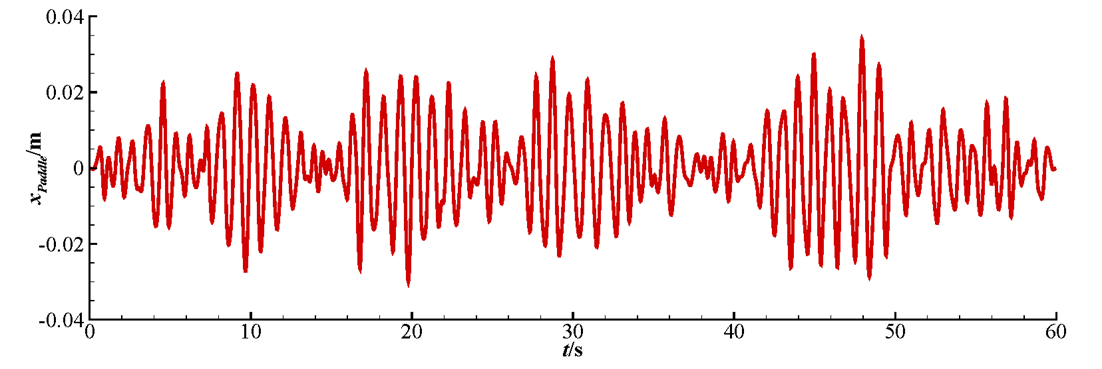
\includegraphics[width=0.8\textwidth]{figures/ch2-wave-setup-irpaddle.png}
  \caption{不规则波的造波机位移时程曲线}
  \label{fig:ch2-wave-setup-irpaddle}
\end{myfigure}
\begin{myfigure}
  
\includegraphics[width=0.8\textwidth]{figures/ch2-wave-setup.png}
  \caption{数值波浪模拟水池设置}
  \label{fig:ch2-wave-setup}
\end{myfigure}

\subsubsection{
  \texorpdfstring{HOS求解器验证} % 正文和目录中显示的标题
  {\thesubsubsection HOS求解器验证} % 书签页中显示的标题
}
\label{sssec:HOS求解器验证}

HOS-NWT在模拟波浪时，对于二维问题需要设置的计算参数主要有以下几个：%
SWEET模型的非线性阶数$i_{\rm{wmk}}$、摄动展开阶数$m_{\rm{HOS}}$、%
波浪场$x$方向上的模态阶数$n_1$和造波机模态阶数$n_3$，%
其中模态数$n_1$和$n_3$一般选取为$(2^k + 1)$，%
更多细节请参考文献\parencite{ducrozetModifiedHighOrderSpectral2012}。%
在本小节的数值波浪模拟中，部分参数参考文献\cite{ducrozetModifiedHighOrderSpectral2012}分别设置为：%
$i_{\rm{wmk}} = 1$，$m_{\rm{HOS}} = 3$，$n_3 = 33$。%
由于$x$方向上模态阶数$n_1$的选取对结果影响较大，下面对其进行收敛性分析，%
分别选取$n_1$为129，257，513和1025进行计算。%
\cref{fig:ch2-wave-HOS-probe1}和\cref{fig:ch2-wave-HOS-probe2}分别给出了在不同参数设置下，%
测点$x_{\rm{probe1}}$和$x_{\rm{probe2}}$处规则波和不规则波的波高结果对比。
\begin{myfigure}
  \begin{subfigure}[b]{0.8\textwidth}
    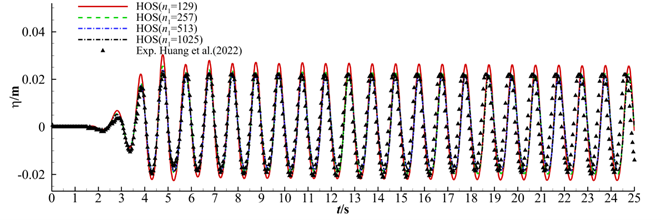
\includegraphics[width=\textwidth]{figures/ch2-wave-HOS-re-probe1.png}
    \caption{规则波}
    \label{ch2-wave-HOS-re-probe1}
  \end{subfigure}
  \begin{subfigure}[b]{0.8\textwidth}
    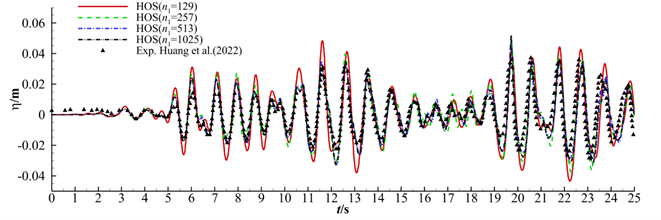
\includegraphics[width=\textwidth]{figures/ch2-wave-HOS-ir-probe1.png}
    \caption{不规则波}
    \label{ch2-wave-HOS-ir-probe1}
  \end{subfigure}
  \caption{$x_{\rm{probe1}}$处的波高：HOS方法结果与文献中试验结果\cite{HuangJiYuXiuZhengGuangHuaLiZiLiuTi2022}对比}
  \label{fig:ch2-wave-HOS-probe1}
\end{myfigure}
\begin{myfigure}
  \begin{subfigure}[b]{0.8\textwidth}
    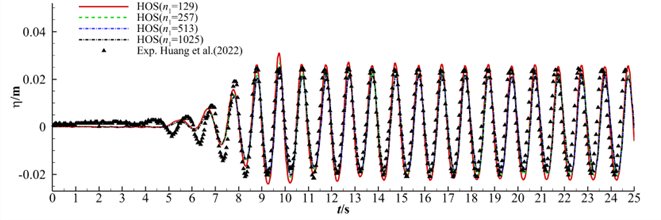
\includegraphics[width=\textwidth]{figures/ch2-wave-HOS-re-probe2.png}
    \caption{规则波}
    \label{ch2-wave-HOS-re-probe2}
  \end{subfigure}
  \begin{subfigure}[b]{0.8\textwidth}
    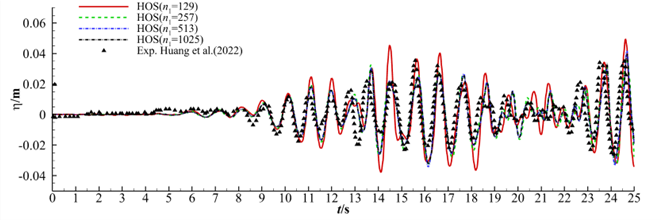
\includegraphics[width=\textwidth]{figures/ch2-wave-HOS-ir-probe2.png}
    \caption{不规则波}
    \label{ch2-wave-HOS-ir-probe2}
  \end{subfigure}
  \caption{$x_{\rm{probe2}}$处的波高：HOS方法结果与文献中试验结果\cite{HuangJiYuXiuZhengGuangHuaLiZiLiuTi2022}对比}
  \label{fig:ch2-wave-HOS-probe2}
\end{myfigure}
\begin{mytable}
  \caption{规则波算例中HOS方法在测点$x_{\rm{probe1}}$处的平均波高对比}
  \label{tab:ch2-wave-HOS-re}
  \begin{tabularx}{\textwidth}{*6{>{\centering\arraybackslash}X}}
    \toprule
    & \multirow{2}{*}{$\bar{\eta}_{\rm{The}}$} & \multicolumn{4}{c}{HOS($n_1$)} \\
    \cline{3-6}
    & & {129} & {257} & {513} & {1025} \\
    \midrule
    {$\bar{\eta}$/m} & {0.04} & {0.04865} & {0.04253} & {0.04053} & {0.04018} \\
    {$\epsilon$/\%} & {——} & {21.63} & {6.33} & {1.33} & {0.45} \\
    \bottomrule
  \end{tabularx}
\end{mytable}

\cref{tab:ch2-wave-HOS-re}中给出了规则波算例中HOS方法结果在测点$x_{\rm{probe1}} = 2.37m$处的平均波高对比，%
其中$\epsilon = \left|\bar{\eta} - \bar{\eta}_{\rm{The}}/\bar{\eta}_{\rm{The}} \times 100\%\right|$，%
$\bar{\eta}$和$\bar{\eta}_{\rm{The}}$分别为HOS方法和理论值在测点处的平均波高。%
结合图表结果可以看出，在规则波算例中随着$n_1$取值增大，%
平均波高逐渐收敛于$\bar{\eta}_{\rm{The}}$，并且当$n_1 = 513$时基本已经收敛。%
从图中不规则波的波高结果中可以看出，当$n_1 = 513$时也基本已经收敛。%

从图表中可以看出HOS方法在模拟规则波和不规则波时，结果收敛后与试验结果吻合比较良好。%
虽然由于其势流方法低数值耗散的特性，在不规则波结果中偶尔会出现波幅略大的情况，但并不影响整体结果的准确性。%
此外需要额外说明，\cref{fig:ch2-wave-HOS-probe1}和\cref{fig:ch2-wave-HOS-probe2}中试验结果随着时间推移逐渐出现了相位偏差，%
这是由于试验过程中的消波处理不够彻底所导致的反射波略微影响了试验结果\cite{HuangJiYuXiuZhengGuangHuaLiZiLiuTi2022}。
% 第5章 总结与展望
\newoddpage % 创建新的奇数页
\section{
  \texorpdfstring{总结与展望} % 正文和目录中显示的标题
  {\thesection 总结与展望} % 书签页中显示的标题
}
\label{sec:总结与展望}

\subsection{
  \texorpdfstring{总结} % 正文和目录中显示的标题
  {\thesubsection 总结} % 书签页中显示的标题
}
\label{ssec:总结}

海洋工程中海上浮式平台在恶劣海况下极易发生波浪砰击、上浪等现象，对人员设备和平台结构可能造成严重危害。%
对于这一类强非线性波浪浮体相互作用问题，CFD数值模拟为了精确捕捉自由液面需要耗费巨大的计算资源。%
本文对势粘流耦合数值方法展开了探索性研究，提出了基于势流方法和无网格SPH方法的势粘流耦合模型。%
文中基于HOS方法、SPH方法和BEM方法，在二维上分别实现了HOS-SPH势粘流单向耦合方法、%
SPH-BEM势粘流双向耦合方法和HOS-SPH-BEM势粘流多模型耦合方法，%
并通过和其他数值方法以及文献中的试验结果对比验证了几类耦合方法的有效性和准确性。%
全文主要结论如下：%

(1)	本文提出了基于势流方法和无网格粒子法的耦合模型。%
该模型通过基于粒子间相互作用的边界条件，实现了势流方法向无网格粒子法速度、压力等流场信息的传递，%
同时基于流量监测网格实现了势粘流耦合过程中拉格朗日粒子法的流入/流出，%
从而实现了流场质量、动量的传递，并和其他数值方法以及试验结果对比验证了该耦合模型的有效性。%

(2)	基于所提出的势粘流耦合模型，本文实现了HOS-SPH单向耦合方法。%
该方法引入了势流HOS方法用于模拟波浪，并且采用耦合模型有效地将势流部分流场信息传递至了粘流部分，从而有效地提高波浪模拟质量和计算效率。%
通过规则波和不规则波模拟、规则波浮体上浪和聚焦波冲击浮体等算例，验证了HOS-SPH单向耦合方法对于计算效率的提高，%
并初步验证了HOS-SPH单向耦合方法对于强非线性波浪结构物相互作用问题的有效性。%
聚焦波冲击浮体算例中耦合方法的数值结果较好地实现了对试验中上浪过程的模拟和复现，并且比较准确地捕捉到了上浪过程中甲板所受到的冲击压力峰值。%

(3)	本文对HOS-SPH单向耦合方法中耦合区域宽度和粘流域宽度这两个重要参数进行了探索，并给出了一些经验参数。%
通过数值波浪模拟算例对不同耦合区域宽度下的结果进行分析，得出耦合区域宽度应选取为$D/\Delta x = 10 \sim 20$，当粒子分辨率较高时该宽度可适当增大。%
通过聚焦波冲击浮体算例对不同粘流域宽度下的结果进行分析，得出在该算例中浮体前端到耦合边界的合适距离约为1.5倍波长，%
而后端到耦合边界的距离约为2倍波长，从而能够保证所关注计算结果的准确性的情况下尽量减少计算成本。%
但由于不同问题中波浪和结构物的尺度、流固耦合的剧烈程度等都有所不同，%
粘流域宽度的选取应视研究问题而定，以保证强非线性现象和粘性效应显著的区域包含在粘流域内。%

(4)	针对单向耦合中耦合边界处反射波的问题，本文实现了SPH-BEM双向耦合方法。%
通过规则波和不规则波模拟，进行了SPH-BEM双向耦合方法的粒子分辨率收敛性分析，并讨论了势流域边界与耦合边界间的距离对波高结果的影响。%
结果表明当势流域边界与耦合边界的距离为2倍波长时波高结果基本收敛。%
波浪数值模拟验证了该方法能够有效地将波浪从SPH粘流域传递到BEM势流域而不在耦合边界上发生反射，从而减小SPH计算域的大小并提高计算效率。%

(5)	在HOS-SPH单向耦合方法和SPH-BEM双向耦合方法的基础上，本文提出了HOS-SPH-BEM多模型耦合方法。%
该方法将势流部分的波浪分解为入射波和辐射绕射波，并分别采用HOS方法和BEM方法求解，%
在保留HOS方法能够高效准确模拟非线性波浪的优势的同时实现了势粘流间的双向耦合。%
在聚焦波冲击浮体算例中，通过与HOS-SPH单向耦合方法结果以及其他结果进行对比，%
验证了HOS-SPH-BEM多模型耦合方法能够减小耦合边界反射波对计算结果的影响，从而进一步提高计算精度。

\subsection{
  \texorpdfstring{创新性工作} % 正文和目录中显示的标题
  {\thesubsection 创新性工作} % 书签页中显示的标题
}
\label{ssec:创新性工作}

本文以恶劣海况下的海上浮式平台为研究背景，针对强非线性波浪浮体相互作用问题中CFD方法难以快速准确计算的难题，%
对势粘流耦合数值方法展开了探索性研究，主要有以下创新性工作：%

(1)	针对波浪与浮体相互作用的数值模拟，提出了基于势流方法与无网格粒子法的耦合模型，初步探索了粘势流场间信息相互传递的难点。%

(2)	自主开发了二维的HOS-SPH单向耦合和HOS-SPH-BEM多模型耦合程序，实现了波浪与浮体相互作用的高效准确模拟。

\subsection{
  \texorpdfstring{展望} % 正文和目录中显示的标题
  {\thesubsection 展望} % 书签页中显示的标题
}
\label{ssec:展望}

本文对波浪和浮体结构物相互作用问题，进行了势粘流耦合方法的初步探索，但仍有大量工作有待开展，以下是作者对此方向的一些展望：%

(1)	本文所实现的HOS-SPH-BEM多模型双向耦合方法中所采用的边界元方法并非全非线性BEM，%
且未分析势粘流耦合过程中的动量、能量机制，因此在后续工作中需要对双向耦合方法进行深入的系统性分析和机理性研究。%

(2)	本文仅在二维上实现了所提出的势粘流耦合方法，且程序仅采用CPU并行运算，暂时难以应用于工程实际中。%
但耦合计算中的边界条件处理方式可以直接推广至三维，并且SPH方法十分适合于GPU并行运算，%
因此未来工作中可将该耦合方法发展至三维并采取GPU并行运算，以适应工程应用中对砰击、上浪等问题的研究。%
此外可以考虑将该耦合方法与水弹性方法等相结合，从而实现对船舶、海上平台等海洋结构物在强非线性波浪作用下的水动力性能进行综合分析。%

(3)	浮式平台波浪砰击、上浪等强非线性问题涉及复杂的气液固耦合现象，而本文并未考虑气相影响，%
并且对于砰击问题的准确预报需要使用更精确的物理模型。%
因此在未来工作中可以采用多相流SPH模型或其他多相流CFD方法进行耦合。


%***********************************************%
%                     参考文献
%***********************************************%
\newoddpage % 创建新的奇数页
\phantomsection % 创建锚点用于超链接
\label{sec:bibliography}
\addcontentsline{toc}{section}{参考文献} % 添加参考文献至目次
\printbibliography[title=参考文献]

%***********************************************%
%                       致谢
%***********************************************%
\newoddpage % 创建新的奇数页
\phantomsection % 创建锚点用于超链接
\section*{致谢}
\label{sec:acknowledgements}
\addcontentsline{toc}{section}{致谢} % 添加致谢至目次

逝者如斯夫，不舍昼夜。
时间从不因人的怠惰或勤奋而停滞，硕士研究生的生涯也如约而至地迎来了尾声。
回顾这两年半，我的心中有许多收获和感慨，也有一些遗憾和叹惋。
这一路走来的经历和成长在这刻悉数浮现脑海，是许多人的陪伴和帮助给予我力量，让我走到了今天。
首先我要感谢我的导师叶永林老师。
第一次见到叶老师时，他便与我相谈许多，从生活到学习，从研究方向到学术作风，
初入二所的我心中的茫然也在老师的温言如玉中逐渐消散。
叶老师对我的谆谆教诲不仅在科研学习上，更在人生态度上，
是他教会了我在迷茫困顿时要坚定信念，不畏困难。
此后的学习生活中，在叶老师的言传身教中，
我逐渐体会了一个科研人应当保持勇于探索、坚定求实的作风和态度，
并且我也努力以这样的标准要求自己。

其次我要感谢我的副导师谢春梅老师。
谢老师在我的学习和生活上给予了我莫大的帮助与关心。
硕士期间，从论文的选题调研和开题，到程序的编写与调试，
以及小论文和大论文的撰写与修改，谢老师都一一悉心教导。
每当我学习上有困难和疑惑时，她都耐心为我解疑答惑，指明方向。
谢老师对学术研究一丝不苟和精益求精的态度成为了我往后在学术道路上的榜样。

感谢中山大学孙鹏楠老师在SPH方法上给我的指导和许多帮助，
当我在SPH方法的理论学习、程序编写和数值模拟中遇到困难时，
孙老师总是不辞辛劳地为我答疑解惑。
还要感谢孙老师课题组的吕鸿冠师兄、管祥善师兄、黄晓婷师姐和徐杨师兄在我学习SPH方法时为我提供的帮助。

感谢部门的程小明老师、朱芸芸老师、倪歆韵研究员、
俞俊博士、王泽博士、王琦彬博士、王思雨博士、郑坤博士、
杨吉师姐、汪敬翔师兄、吴凡蕾师姐、魏子阳师兄、屈毫拓师兄等人在我读研期间对我的关心和照顾。感谢大家。

感谢研究生部副主任王丽艳老师和叶荫老师为我读研期间的学习生活提供的许多帮助。
同时也感谢我来到二所认识的2021级同学们，他们在我生病时的照顾、失意时的鼓励、落寞时的陪伴都让我铭记于心。
还要感谢余昕师兄在我学习生活中一直以来的帮助。感谢大家。

感谢各位专家教授在百忙之中对我的论文进行评审并提供宝贵的意见。

最后感谢我挚爱的父母，感谢你们一直以来的无私奉献与默默支持，给了我不断前进的动力，
同时由衷感谢我身边的朋友与亲人们，你们的关怀使我倍受鼓舞，你们的帮助使我渡过难关，不断进步。

%***********************************************%
%                学术论文和科研成果目录
%***********************************************%
\newoddpage % 创建新的奇数页
\section*{学术论文和科研成果目录}
\label{sec:achievements}
\phantomsection % 创建锚点用于超链接
\addcontentsline{toc}{section}{学术论文和科研成果目录} % 添加学术论文和科研成果目录至目次

\begin{enumerate}[label={[\arabic*]}]
  \item XIE C M, \textbf{YANG J C}, SUN P N, et al. %
  An accurate and efficient HOS-meshfree CFD coupling method for %
  simulating strong nonlinear wave–body interactions[J]. %
  Ocean Engineering, 2023, 287: 115889. \textbf{(已发表)}
  \item 叶永林, \textbf{杨军城}, 谢春梅, 等. %
  面向船海水动力应用的势粘流耦合方法研究综述[J]. %
  船舶力学, 2024, 28(04): 606-625. \textbf{(已发表)}
\end{enumerate}

\end{document}